\PassOptionsToPackage{unicode=true}{hyperref} % options for packages loaded elsewhere
\PassOptionsToPackage{hyphens}{url}
%
\documentclass[]{article}
\usepackage{lmodern}
\usepackage{amssymb,amsmath}
\usepackage{ifxetex,ifluatex}
\usepackage{fixltx2e} % provides \textsubscript
\ifnum 0\ifxetex 1\fi\ifluatex 1\fi=0 % if pdftex
  \usepackage[T1]{fontenc}
  \usepackage[utf8]{inputenc}
  \usepackage{textcomp} % provides euro and other symbols
\else % if luatex or xelatex
  \usepackage{unicode-math}
  \defaultfontfeatures{Ligatures=TeX,Scale=MatchLowercase}
\fi
% use upquote if available, for straight quotes in verbatim environments
\IfFileExists{upquote.sty}{\usepackage{upquote}}{}
% use microtype if available
\IfFileExists{microtype.sty}{%
\usepackage[]{microtype}
\UseMicrotypeSet[protrusion]{basicmath} % disable protrusion for tt fonts
}{}
\IfFileExists{parskip.sty}{%
\usepackage{parskip}
}{% else
\setlength{\parindent}{0pt}
\setlength{\parskip}{6pt plus 2pt minus 1pt}
}
\usepackage{hyperref}
\hypersetup{
            pdftitle={Un cours sur les indices des prix},
            pdfauthor={Steve Martin},
            pdfborder={0 0 0},
            breaklinks=true}
\urlstyle{same}  % don't use monospace font for urls
\usepackage[margin=1in]{geometry}
\usepackage{color}
\usepackage{fancyvrb}
\newcommand{\VerbBar}{|}
\newcommand{\VERB}{\Verb[commandchars=\\\{\}]}
\DefineVerbatimEnvironment{Highlighting}{Verbatim}{commandchars=\\\{\}}
% Add ',fontsize=\small' for more characters per line
\usepackage{framed}
\definecolor{shadecolor}{RGB}{248,248,248}
\newenvironment{Shaded}{\begin{snugshade}}{\end{snugshade}}
\newcommand{\AlertTok}[1]{\textcolor[rgb]{0.94,0.16,0.16}{#1}}
\newcommand{\AnnotationTok}[1]{\textcolor[rgb]{0.56,0.35,0.01}{\textbf{\textit{#1}}}}
\newcommand{\AttributeTok}[1]{\textcolor[rgb]{0.77,0.63,0.00}{#1}}
\newcommand{\BaseNTok}[1]{\textcolor[rgb]{0.00,0.00,0.81}{#1}}
\newcommand{\BuiltInTok}[1]{#1}
\newcommand{\CharTok}[1]{\textcolor[rgb]{0.31,0.60,0.02}{#1}}
\newcommand{\CommentTok}[1]{\textcolor[rgb]{0.56,0.35,0.01}{\textit{#1}}}
\newcommand{\CommentVarTok}[1]{\textcolor[rgb]{0.56,0.35,0.01}{\textbf{\textit{#1}}}}
\newcommand{\ConstantTok}[1]{\textcolor[rgb]{0.00,0.00,0.00}{#1}}
\newcommand{\ControlFlowTok}[1]{\textcolor[rgb]{0.13,0.29,0.53}{\textbf{#1}}}
\newcommand{\DataTypeTok}[1]{\textcolor[rgb]{0.13,0.29,0.53}{#1}}
\newcommand{\DecValTok}[1]{\textcolor[rgb]{0.00,0.00,0.81}{#1}}
\newcommand{\DocumentationTok}[1]{\textcolor[rgb]{0.56,0.35,0.01}{\textbf{\textit{#1}}}}
\newcommand{\ErrorTok}[1]{\textcolor[rgb]{0.64,0.00,0.00}{\textbf{#1}}}
\newcommand{\ExtensionTok}[1]{#1}
\newcommand{\FloatTok}[1]{\textcolor[rgb]{0.00,0.00,0.81}{#1}}
\newcommand{\FunctionTok}[1]{\textcolor[rgb]{0.00,0.00,0.00}{#1}}
\newcommand{\ImportTok}[1]{#1}
\newcommand{\InformationTok}[1]{\textcolor[rgb]{0.56,0.35,0.01}{\textbf{\textit{#1}}}}
\newcommand{\KeywordTok}[1]{\textcolor[rgb]{0.13,0.29,0.53}{\textbf{#1}}}
\newcommand{\NormalTok}[1]{#1}
\newcommand{\OperatorTok}[1]{\textcolor[rgb]{0.81,0.36,0.00}{\textbf{#1}}}
\newcommand{\OtherTok}[1]{\textcolor[rgb]{0.56,0.35,0.01}{#1}}
\newcommand{\PreprocessorTok}[1]{\textcolor[rgb]{0.56,0.35,0.01}{\textit{#1}}}
\newcommand{\RegionMarkerTok}[1]{#1}
\newcommand{\SpecialCharTok}[1]{\textcolor[rgb]{0.00,0.00,0.00}{#1}}
\newcommand{\SpecialStringTok}[1]{\textcolor[rgb]{0.31,0.60,0.02}{#1}}
\newcommand{\StringTok}[1]{\textcolor[rgb]{0.31,0.60,0.02}{#1}}
\newcommand{\VariableTok}[1]{\textcolor[rgb]{0.00,0.00,0.00}{#1}}
\newcommand{\VerbatimStringTok}[1]{\textcolor[rgb]{0.31,0.60,0.02}{#1}}
\newcommand{\WarningTok}[1]{\textcolor[rgb]{0.56,0.35,0.01}{\textbf{\textit{#1}}}}
\usepackage{longtable,booktabs}
% Fix footnotes in tables (requires footnote package)
\IfFileExists{footnote.sty}{\usepackage{footnote}\makesavenoteenv{longtable}}{}
\usepackage{graphicx,grffile}
\makeatletter
\def\maxwidth{\ifdim\Gin@nat@width>\linewidth\linewidth\else\Gin@nat@width\fi}
\def\maxheight{\ifdim\Gin@nat@height>\textheight\textheight\else\Gin@nat@height\fi}
\makeatother
% Scale images if necessary, so that they will not overflow the page
% margins by default, and it is still possible to overwrite the defaults
% using explicit options in \includegraphics[width, height, ...]{}
\setkeys{Gin}{width=\maxwidth,height=\maxheight,keepaspectratio}
\setlength{\emergencystretch}{3em}  % prevent overfull lines
\providecommand{\tightlist}{%
  \setlength{\itemsep}{0pt}\setlength{\parskip}{0pt}}
\setcounter{secnumdepth}{5}
% Redefines (sub)paragraphs to behave more like sections
\ifx\paragraph\undefined\else
\let\oldparagraph\paragraph
\renewcommand{\paragraph}[1]{\oldparagraph{#1}\mbox{}}
\fi
\ifx\subparagraph\undefined\else
\let\oldsubparagraph\subparagraph
\renewcommand{\subparagraph}[1]{\oldsubparagraph{#1}\mbox{}}
\fi

% set default figure placement to htbp
\makeatletter
\def\fps@figure{htbp}
\makeatother


\title{Un cours sur les indices des prix}
\author{Steve Martin}
\date{Mai 2020}

\begin{document}
\maketitle

{
\setcounter{tocdepth}{2}
\tableofcontents
}
\hypertarget{aperuxe7u}{%
\section*{Aperçu}\label{aperuxe7u}}
\addcontentsline{toc}{section}{Aperçu}

Ce cours donne une introduction moderne et simple aux indices des prix. L'accent mis sur les principales idées et concepts qui sont importants pour les utilisateurs et les compilateurs d'indices de prix; par conséquent, le cours n'est pas encyclopédique et plusieurs sujets importants sont soit traités rapidement, soit pas du tout traités. De nombreuses références sont fournies pour compléter le matériel de ce cours et étendre la portée des sujets traités. Dans l'ensemble, le cours repose fermement sur le domaine de la théorie et est conçu pour aider à favoriser la compréhension de ce qu'est un indice des prix. Plusieurs exemples pratiques utilisant le langage de programmation R sont donnés tout au long du cours, ainsi que plusieurs exercices appliqués. Mais la plupart des aspects les plus «réels» de l'élaboration d'un indice des prix sont ignorés. Ce n'est pas parce que ces choses ne sont pas importantes; il est plutôt difficile d'apprécier ces sujets plus pratiques sans une solide compréhension de la théorie.

Le cours est divisé en quatre modules qui s'appuient les uns sur les autres. Le premier module donne une introduction aux indices de prix, en se concentrant principalement sur les aspects informatiques d'un indice de prix. Le deuxième module donne une large introduction à la théorie des indices des prix, en mettant l'accent sur la motivation des indices des prix qui sont produits par les organismes statistiques nationaux. Le troisième module couvre les ajustements de qualité, l'un des principaux obstacles pratiques lors de la construction d'un indice des prix. Le quatrième module rassemble le tout avec un exercice étendu pour construire et analyser un indice des prix avec R.

\hypertarget{part-introduction-aux-indices-de-prix}{%
\part{Introduction aux indices de prix}\label{part-introduction-aux-indices-de-prix}}

\hypertarget{programme}{%
\section{Programme}\label{programme}}

Un indice des prix permet de condenser systématiquement les informations sur de nombreux prix pour une gamme de produits et services en une seule valeur. Les indices des prix sont largement utilisés pour analyser et comparer les conditions macroéconomiques dans le temps et ont des implications importantes pour les politiques gouvernementales.

L'objectif de ce module est de fournir une introduction aux indices de prix, avec une application aux indices de prix des entrées et sorties de production (indice des prix à la production), et des prix à la consommation (indice des prix à la consommation). À la fin du module, une personne devrait:

\begin{enumerate}
\def\labelenumi{\arabic{enumi}.}
\item
  Comprendre les raisons pour lesquelles les indices de prix sont compilés et pourquoi ils sont importants.
\item
  Familiarisez-vous avec les formules d'index communes et comment les manipuler.
\item
  Avoir une compréhension de base de la structure d'un indice de prix et de son calcul.
\end{enumerate}

Ce module est utile à la fois pour les utilisateurs et les compilateurs d'indices de prix ayant peu de connaissances préalables sur les utilisations et la construction d'un indice de prix.

Ce module se compose de lectures autodirigées, accompagnées d'un devoir. Au total, environ 10 à 15 heures devraient être consacrées à ce module

Il n'y a pas de prérequis pour ce module, bien que les individus devraient être à l'aise avec l'algèbre de base et les arguments mathématiques simples. Un cours d'introduction à la macroéconomie est utile.

L'évaluation de ce module est basée sur une tâche composée de 20 questions à choix multiples / vrai-faux qui s'appuient sur du matériel dans le contenu du cours et les lectures. La collaboration sur la mission est la bienvenue, mais chaque personne doit soumettre son propre travail unique. La réussite de ce module nécessite au moins 65\% sur l'affectation.

Les lectures de ce module proviennent des chapitres 1, 2, 4 et 9 du Manuel de l'indice des prix à la production (ILO et al. 2004b) et / ou du Manuel de l'indice des prix à la consommation (ILO et al. 2004a), publiés par le FMI (disponibles gratuitement sur leur site Web). Comme il existe un chevauchement considérable entre ces sources, le manuel PPI est utilisé comme référence principale.

Veuillez envoyer un e-mail à l'instructeur du cours si vous avez des questions ou si vous avez besoin d'aide concernant le matériel ou le devoir du cours.

\hypertarget{quest-ce-quun-indice-des-prix-et-pourquoi-en-avons-nous-besoin}{%
\section{Qu'est-ce qu'un indice des prix et pourquoi en avons-nous besoin?}\label{quest-ce-quun-indice-des-prix-et-pourquoi-en-avons-nous-besoin}}

Un indice des prix est un outil pour mesurer l'évolution du prix des biens et services au fil du temps. Les indices des prix ont une longue histoire et constituent une statistique macroéconomique importante et largement utilisée. Cette section du cours commence par présenter ce qu'est un indice des prix, à quoi ils servent et pourquoi un indice des prix est nécessaire.

📖 Manuel PPI: Chapitre 1, sections A, K; Chapitre 2, sections A, B, D1, D2, E, F.

📖 Manuel de l'IPC: chapitre 1, paragraphes 1.8 à 1.12; Chapitre 2.

\hypertarget{quest-ce-quun-indice-des-prix}{%
\subsection{Qu'est-ce qu'un indice des prix?}\label{quest-ce-quun-indice-des-prix}}

Un indice de prix est une série chronologique économique qui donne la variation en pourcentage des prix d'une collection de biens et services entre un moment donné et un point de référence fixe (c'est-à-dire la période de base ou la période de référence).\footnote{Un prix l'indice peut également être utilisé pour mesurer la différence de prix à différents endroits au même moment, bien qu'il s'agisse d'une utilisation moins courante d'un indice de prix.} Un indice de prix est généralement représenté de manière à soustraire 100 de la valeur de l'indice donne la variation en pourcentage des prix des biens et services capturés par l'indice. Par exemple, si un indice des prix des widgets a une valeur de 110 pendant une certaine période, alors les prix des widgets ont augmenté de 10\% depuis la période de base. Cette représentation signifie également que l'indice a une valeur de 100 dans la période de base.

Le graphique ci-dessous donne un exemple d'indice de prix mensuel montrant la variation des prix de chaque mois de l'année par rapport à janvier (la période de base), de sorte que chaque point du graphique donne la variation en pourcentage des prix depuis janvier. Par exemple, en mars, l'indice avait une valeur de 103, ce qui signifie que les prix ont augmenté de 3\% entre mars et janvier, tandis que l'indice avait une valeur de 99 en juin, ce qui signifie que les prix ont diminué de 1\% entre janvier et juin.

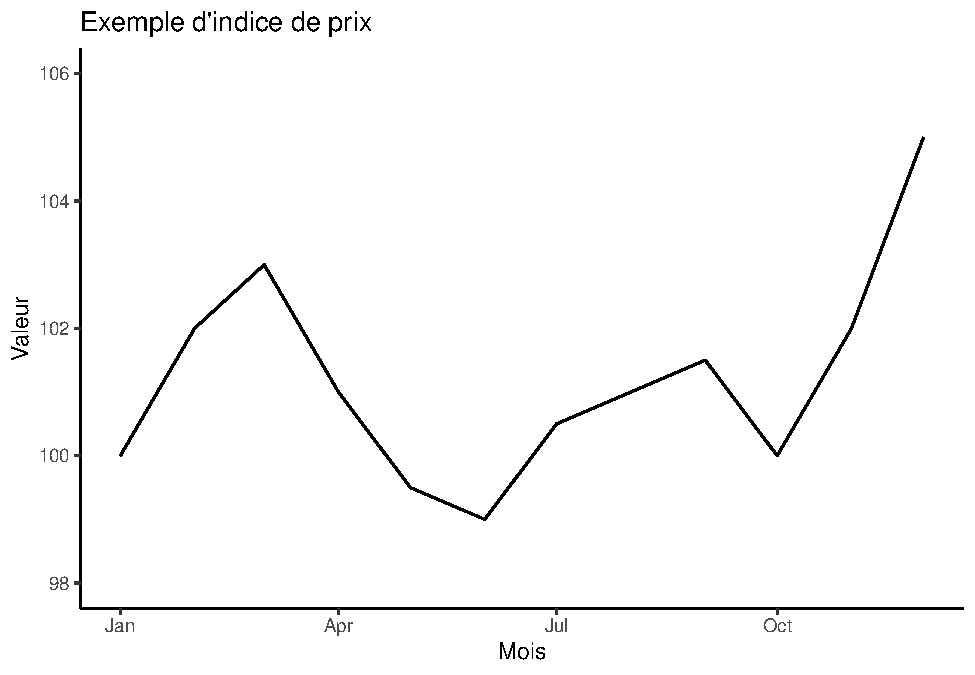
\includegraphics{cours-indices-des-prix_files/figure-latex/unnamed-chunk-1-1.pdf}

Étant donné qu'un indice des prix ne mesure que la variation relative des prix depuis la période de base, le changement d'échelle de l'indice ne modifie pas son contenu économique. Par exemple, la division de 100 de toutes les valeurs du graphique ci-dessus ne modifie pas la forme du graphique ou la variation en pourcentage de la valeur d'index qui en résulte depuis la période de base. C'est pour cette raison que l'ampleur d'un indice des prix ne donne pas une mesure du niveau des prix à un moment donné - un indice des prix ne peut que mesurer la variation des prix au fil du temps.

L'utilité d'un indice des prix est qu'il permet de condenser systématiquement les informations sur de nombreux prix pour une gamme de biens et services en une seule valeur qui mesure l'évolution des prix de ces biens et services au fil du temps. Bien que les biens et services qui entrent dans la portée d'un indice des prix dépendent de son objet, tous les indices des prix donnent une mesure des mouvements de prix agrégés pour un ensemble bien défini de produits. Cela donne à son tour une mesure des pressions inflationnistes dans une économie et, par conséquent, les indices des prix sont omniprésents lors de l'examen des conditions et des politiques macroéconomiques.

\hypertarget{utilisations-dun-indice-des-prix}{%
\subsection{Utilisations d'un indice des prix}\label{utilisations-dun-indice-des-prix}}

Dans la pratique, il existe deux grandes catégories dans lesquelles les indices des prix publiés par les organismes statistiques nationaux entrent dans la catégorie: les indices des prix à la consommation (IPC) et les indices des prix à la production (IPP). Comme leur nom l'indique, les IPC sont axés sur la mesure des variations de prix des biens et services achetés par les consommateurs (consommation finale), tandis que les IPP se concentrent sur la mesure des prix facturés par les producteurs pour les biens et services produits et les prix payés pour les intrants dans la production. Malgré les nombreuses subtilités sur ce qui constitue un consommateur et ce qui constitue un producteur, les IPC et les IPP cherchent à mesurer la variation des prix au fil du temps pour les biens et services qui sont négociés dans une économie. Par conséquent, il y a souvent
chevauchement considérable dans la façon dont les IPC et les IPP sont calculés et utilisés, et il n'est pas nécessaire de faire la distinction entre un indice comme un IPC ou un IPP --- il suffit souvent de parler d'un indice général des prix.

L'utilisation la plus importante d'un indice des prix, qu'il s'agisse d'un IPC ou d'un IPP, est probablement de mesurer l'inflation - le changement systématique des prix dans une économie au fil du temps. Au-delà d'être un indicateur macroéconomique important, la mesure de l'inflation affecte directement de nombreuses interactions économiques dans les économies modernes. Par exemple, de nombreuses banques centrales opèrent dans un régime de ciblage de l'inflation, selon lequel la politique monétaire est menée en partie pour maintenir le taux d'inflation dans une fourchette prédéterminée (par exemple, 1\% à 3\% par an). Ce régime politique nécessite une mesure fréquente et opportune de l'inflation, et l'instrument utilisé pour mesurer l'inflation peut avoir un impact direct sur la politique monétaire et, par conséquent, sur les taux d'intérêt. L'inflation affecte également les salaires et les contrats de services, les paiements de pension et les prestations de sécurité sociale, car ces contrats sont souvent indexés sur l'inflation --- si les prix augmentent de 2\% par an, les salaires augmentent également de 2\% par an. L'indexation préserve la valeur des paiements au fil du temps sans avoir à constamment renégocier les contrats ou repenser les politiques. La mesure de l'inflation a donc des implications importantes sur le revenu des ménages et les revenus de l'industrie.

Au-delà de la mesure de l'inflation, l'une des principales utilisations des indices de prix pour les organismes statistiques nationaux est de déflater les valeurs agrégées dans un cadre de comptabilité nationale pour obtenir une mesure de l'évolution de la production de biens et services réels au fil du temps. Cela équivaut à trouver un indice de quantité pour condenser systématiquement les informations sur de nombreuses sorties pour une gamme de biens et services en une seule valeur qui mesure la variation de la quantité de biens et services produits au fil du temps. Bien qu'il existe de nombreux détails, la justification de la déflation des valeurs agrégées pour obtenir une mesure de la production réelle est assez simple. Si \(V_1 / V_0\) est le rapport entre la valeur de la production de la période 1 et la valeur de la production de la période 0, et si cela peut être décomposé en un indice de quantité \(Q\) et un indice de prix \(I\) tels que \(V_1 / V_0 = IQ\), alors la variation de la production réelle entre la période 0 et la période 1 est simplement \(Q = V_1 / (V_0 I)\). L'évolution de la valeur de la production au fil du temps - une quantité connue - peut être transformée en une mesure de l'évolution de la production réelle en la déflatant simplement avec un indice des prix.

\hypertarget{pourquoi-un-indice-des-prix}{%
\subsection{Pourquoi un indice des prix?}\label{pourquoi-un-indice-des-prix}}

Le point de départ pour comprendre l'utilité d'un indice des prix est de reconnaître qu'il n'y en a pas besoin si l'objectif est de comparer le prix d'un seul bien ou service au cours d'une période au prix du même bien ou service au cours d'une autre période. Si \(p_1\) est le prix d'un bien pendant la période 1 et \(p_0\) est le prix de ce même bien pendant la période 0, alors le prix relatif \(p_1 / p_0\) donne sans ambiguïté la variation en pourcentage du prix entre la période 1 et la période 0 La nécessité d'un indice des prix découle d'un problème fondamental de comparaison d'une collecte de deux prix ou plus à deux moments pour arriver à une variation globale des prix.

Pour illustrer ce problème de comparaison, supposons qu'il existe deux biens, notés \(i\) et \(j\), qui se vendent dans les périodes 0 et 1. Si le prix du bon \(i\) et le prix du bon \(j\) augmentent tous les deux entre les périodes 0 et la période 1, il n'est donc pas contesté de dire que les prix ont augmenté entre la période 0 et la période 1 (même si la quantité de prix a augmenté moins clairement). De même, si les deux prix baissent, il est naturel de dire que les prix ont baissé. Cependant, un problème se pose si le prix du bon \(i\) augmente entre la période 0 et
période 1 tandis que le prix du bon \(j\) diminue. Dans ce cas, il n'est pas clair si les prix ont augmenté ou diminué --- il n'y a pas de moyen évident de donner une direction unique à l'évolution des prix au fil du temps.

Une solution à ce problème de comparaison consiste à trouver un moyen d'agréger les prix relatifs pour de nombreux biens et services pour former un ratio unique, qui est ensuite interprété comme l'évolution globale des prix au fil du temps. C'est le travail d'un indice des prix. Bien qu'un indice des prix résout le problème de la comparaison, il introduit un nouveau défi: comment combiner au mieux les prix relatifs pour produire une mesure unique décrivant la variation globale des prix. Par conséquent, diverses formules d'indice-nombre ont été proposées pour construire un indice de prix.

\hypertarget{formule-de-numuxe9ro-dindex}{%
\section{Formule de numéro d'index}\label{formule-de-numuxe9ro-dindex}}

Il existe un grand nombre de formules d'indices qui peuvent être utilisées pour combiner des informations sur les prix à deux moments dans le temps pour produire un indice des prix, malgré l'objectif commun de mesurer les variations de prix au fil du temps. Cette section du cours couvre 10 formules d'indice-nombre importantes qui sont utilisées dans la pratique pour calculer un indice de prix. Le nom de la personne qui l'a développée est associé à chaque formule. Il est important d'associer les noms aux formules, car ils sont généralement désignés par leur nom dans l'application. Il s'agit malheureusement d'un exercice de mémorisation, car la plupart des formules d'index ont une forme similaire.

Pour aider à construire l'intuition et une compréhension plus approfondie de ce que font les formules de l'indice-nombre, ces différentes approches pour calculer un indice de prix peuvent être classées en gros comme des indices de prix arithmétiques ou des indices de prix géométriques. Toutes les formules de nombre d'index ne tombent pas dans ces deux groupes --- par exemple, il existe également des indices de prix harmoniques, une catégorie qui peut chevaucher des indices arithmétiques --- mais les indices arithmétiques et géométriques sont assez faciles à comprendre, avec la plupart des indices- formules de nombres entrant dans l'une de ces deux catégories.

En pratique, un indice de prix est multiplié par 100, de sorte que le changement en pourcentage de la valeur de l'indice sur deux périodes est simplement la valeur de l'indice moins 100. Il s'agit simplement d'une normalisation pratique qui n'a aucune incidence sur le contenu économique d'un indice de prix, et est ignoré dans cette section. Notez que toutes les formules d'index peuvent être multipliées par 100 pour les mettre sur l'échelle habituelle.

📖 Manuel PPI: Chapitre 1, sections B1 - B3.

\hypertarget{indices-arithmuxe9tiques-des-prix}{%
\subsection{Indices arithmétiques des prix}\label{indices-arithmuxe9tiques-des-prix}}

Un indice arithmétique des prix prend les prix relatifs pour une collection de biens et services sur deux périodes et les combine ensemble comme moyenne pondérée. Autrement dit, un indice arithmétique est simplement la variation moyenne du prix entre deux points dans le temps. Laissant les marchandises être énumérées par \(i = 1, \ldots, n\), un index arithmétique entre la période 0 et la période 1 a la forme générale\footnote{La lettre majuscule sigma \(\Sigma\) est l'opérateur de sommation. Pour une collection de nombres \(x_{1}, x_{2}, \ldots, x_{n}\), \(\sum_{i = 1}^{n} x_{i}\) signifie \(x_{1} + x_{2} + \ldots + x_{n}\).}

\begin{align*}
I^{A} = \sum_{i = 1}^{n} \omega_{i} \frac{p_{i1}}{p_{i0}},
\end{align*}

où \(p_{it}\) est le prix du bon \(i\) dans la période \(t = 0,1\), et \(\omega_{i} \geq 0\) est le poids que le bon \(i\) reçoit dans le calcul de l'indice, tel que \(\sum_{i = 1}^{n} \omega_{i} = 1\).

Différents indices de prix arithmétiques correspondent à des cas particuliers de l'indice arithmétique général, selon le choix des pondérations. La plupart de ces choix utilisent des informations sur la quantité d'un bien vendu, de sorte que les poids donnent une mesure de l'importance économique d'un bien. Notons \(q_{it}\) la quantité de bon \(i\) consommée / produite dans la période \(t = 0,1\).

Avant d'examiner des indices arithmétiques spécifiques, il convient de noter qu'un indice arithmétique peut toujours être écrit comme le rapport des dépenses / recettes pour un ``panier'' de biens et services à deux points dans le temps, de sorte que pour tout ensemble de pondérations, il est implicite ``quantités'' telles que

\begin{align*}
I^{A} = \frac{\sum_{i = 1}^{n} p_{i1} \tilde{q}_{i}}{\sum_{i = 1}^{n} p_{i0} \tilde{q}_{i}},
\end{align*}

où \(\tilde{q}_{i} = \alpha \omega_{i} / p_{i0}\) pour un certain facteur de proportionnalité \(\alpha\).\footnote{La valeur de \(\alpha\) n'a aucun impact sur l'indice, mais est nécessaire pour que la propriété interprète \(\tilde{q}_{i}\) comme une quantité. Par exemple, si \(\omega_{i}\) est la part des dépenses de la période 0 sur les bons \(i\), \(p_{i0} q_{i0} / \sum_{j = 1}^{n} p_{j0} q_{j0}\), puis \(\alpha = \sum_{j = 1}^{n} p_{j0} q_{j0}\) pour que \(\tilde{q}_{i} = q_{i0}\).} Ainsi, un indice arithmétique peut toujours être interprété comme le rapport des dépenses nécessaires à l'achat d'un panier fixe de biens à deux moments (ou les revenus d'un panier fixe de biens à deux moments). Le choix du panier est lié un à un au choix des pondérations utilisées pour agréger les prix relatifs. Les deux représentations de l'indice arithmétique sont utilisées, car certains indices sont plus faciles à représenter sous une forme que l'autre.

\hypertarget{indices-arithmuxe9tiques-communs}{%
\subsection{Indices arithmétiques communs}\label{indices-arithmuxe9tiques-communs}}

Il existe six principaux indices de prix arithmétiques qui sont utilisés dans la pratique, chacun correspondant à une déclaration différente sur le poids qu'un prix relatif devrait recevoir dans le calcul de l'indice.

\textbf{Indice Carli}. La définition de \(\omega_{i} = 1 / n\) entraîne l'index Carli

\begin{align*}
I^{A}_{C} = \frac{1}{n} \sum_{i = 1}^{n} \frac{p_{i1}}{p_{i0}}.
\end{align*}

L'indice Carli adopte une position neutre sur les pondérations et considère chaque prix relatif comme tout aussi important.

\textbf{Indice de Dutot}. La définition de \(\omega_{i} = p_{i0} / \sum_{j = 1}^{n} p_{j0}\) entraîne l'index Dutot

\begin{align*}
I^{A}_D = \frac{\sum_{i = 1}^{n} p_{i1}}{\sum_{i = 1}^{n} p_{i0}}.
\end{align*}

L'indice Dutot donne plus de poids aux prix apparentés qui ont un prix supérieur à la période 0, en comparant le prix moyen des biens de la période 1 au prix moyen de la période 0.

\textbf{Indice Lowe}. La définition de \(\omega_{i} = p_{i0} q_{ib} / \sum_{j = 1}^{n} p_{j0} q_{jb}\) entraîne l'index Lowe

\begin{align*}
I^{A}_{l} = \frac{\sum_{i = 1}^{n} p_{i1} q_{ib}}{\sum_{i = 1}^{n} p_{i0} q_{ib}},
\end{align*}

où \(q_{ib}\) est la quantité de bons \(i\) au cours d'une période de base \(b\), généralement avant la période 0. Les pondérations de l'indice de Lowe sont des parts de dépenses / revenus ``hybrides'' pour le panier de biens et services dans la période \(b\) en utilisant les prix de la période 0.

\textbf{Indice de Laspeyres}. La définition de \(\omega_{i} = p_{i0} q_{i0} / \sum_{j = 1}^{n} p_{j0} q_{j0}\) entraîne l'index de Laspeyres

\begin{align*}
I^{A}_{L} = \frac{\sum_{i = 1}^{n} p_{i1} q_{i0}}{\sum_{i = 1}^{n} p_{i0} q_{i0}}.
\end{align*}

L'indice de Laspeyres pondère les prix relatifs en fonction de leur part des dépenses / recettes pour la période 0, et constitue un cas particulier de l'indice de Lowe.

\textbf{Indice de Paasche}. La définition de \(\omega_{i} = p_{i0} q_{i1} / \sum_{j = 1}^{n} p_{j0} q_{j1}\) entraîne l'index de Paasche

\begin{align*}
I^{A}_{P} = \frac{\sum_{i = 1}^{n} p_{i1} q_{i1}}{\sum_{i = 1}^{n} p_{i0} q_{i1}}.
\end{align*}

Comme l'indice Laspeyres, l'indice Paasche est un cas particulier de l'indice Lowe et utilise des parts hybrides dépenses / recettes pour pondérer les prix relatifs.

Il convient de noter que l'indice de Paasche est souvent calculé comme une moyenne harmonique pondérée, avec des parts de dépenses / recettes de la période 1 comme pondérations, de sorte que

\begin{align*}
I^{A}_{P} = \left (\sum_{i = 1}^{n} \frac{\frac{p_{i1} q_{i1}}{\sum_{j = 1}^{n} p_{j1} q_{j1}}}{\frac{p_{i1}}{p_{i0}}} \right)^{- 1}.
\end{align*}

Il s'agit d'un exemple d'indice de prix harmonique et d'un moyen pratique de calculer un indice de Paasche si seules les parts des dépenses / recettes de la période 1 sont connues, plutôt que les quantités de la période 1.

\textbf{Indice Young}. La définition de \(\omega_{i} = p_{ib} q_{ib} / \sum_{j = 1}^{n} p_{jb} q_{jb}\) entraîne l'index Young

\begin{align*}
I^{A}_{Y} = \sum_{i = 1}^{n} \frac{p_{ib} q_{ib}}{\sum_{j = 1}^{n} p_{jb} q_{jb}} \frac{p_{i1}}{p_{i0}},
\end{align*}

où \$ q\_\{ib\}\$ est la quantité de bon \(i\) dans une période de base \(b\), avec \$ p\_\{ib\}\$ comme prix, généralement avant la période 0. L'indice Young utilise la période \(b\) dépenses / parts de revenus sous forme de pondérations.\footnote{Dans certains cas, un indice de Young est utilisé pour faire référence à un indice arithmétique général, plutôt qu'à un indice arithmétique avec un ensemble particulier de pondérations.} L'indice Laspeyres est un cas particulier de l'indice Young.

Dans la plupart des applications, un indice de Laspeyres est la formule d'indice-nombre souhaitée pour un indice de prix arithmétique, en partie parce que les pondérations peuvent être observées séparément des informations sur les prix. Les pondérations pour un IPC, par exemple, peuvent provenir d'une enquête nationale représentative des dépenses des ménages, et donc seules les informations sur les prix doivent être collectées pour calculer un indice de Laspeyres. Bien que les pondérations de Young soient également directement observables, elles ne reflètent pas nécessairement les changements dans la composition des dépenses ou des sources de revenus entre la période \(b\) et la période 0. Alternativement, les indices Lowe et Paasche ont tous deux des pondérations qui doivent être explicitement calculées . Comme l'indice Young, l'indice Lowe utilise des informations de quantité obsolètes, tandis que l'indice Paasche utilise des informations de quantité de la période actuelle, ce qui signifie généralement qu'il ne peut pas être calculé en temps opportun.

Malgré l'objectif de calculer un indice de Laspeyres, dans la plupart des applications, un indice arithmétique est souvent calculé comme un indice de Young (ou parfois un indice de Lowe), car il est difficile d'obtenir des informations en temps opportun sur le partage des dépenses / recettes. L'attente des informations de pondération peut nécessiter de retarder la production d'un indice bien après la période 0. L'espoir est que les pondérations utilisées dans l'indice de Young offrent une approximation raisonnable des pondérations de Laspeyres.

\hypertarget{indices-arithmuxe9tiques-moins-courants}{%
\subsection{Indices arithmétiques moins courants}\label{indices-arithmuxe9tiques-moins-courants}}

Il existe une variété d'indices arithmétiques qui sont rarement utilisés dans la pratique, mais peuvent être utiles à connaître. Comme ces formules d'index sont rarement utilisées, ce matériau peut être sauté en toute sécurité.

\textbf{Indice de Palgrave}. La définition de \(\omega_{i} = p_{i1} q_{i1} / \sum_{j = 1}^{n} p_{j1} q_{j1}\) entraîne l'index Palgrave

\begin{align*}
I^{A}_{p} = \sum_{i = 1}^{n} \frac{p_{i1} q_{i1}}{\sum_{j = 1}^{n} p_{j1} q_{j1}} \frac{p_{i1}}{p_{i0}}.
\end{align*}

L'indice Palgrave utilise les parts de dépenses de la période 1 comme pondérations et constitue un cas particulier de l'indice Young.

\textbf{Index sans nom}. Réglage

\begin{align*}
\omega_{i} = \frac{1}{2} \frac{p_{i0} q_{i0}}{\sum_{j = 1}^{n} p_{j0} q_{j0}} + \frac{1}{2} \frac{p_{i1} q_{i1}}{\sum_{j = 1}^{n} p_{j1} q_{j1}}
\end{align*}

donne une formule de numéro d'index sans nom,

\begin{align*}
I^{A}_{U} = \sum_{i = 1}^{n} \left(\frac{1}{2} \frac{p_{i0} q_{i0}}{\sum_{j = 1}^{n} p_{j0} q_{j0}} + \frac{1}{2} \frac{p_{i1} q_{i1}}{\sum_{j = 1}^{n} p_{j1} q_{j1}} \right) \frac{p_{i1}}{p_{i0}}.
\end{align*}

Cet indice est un mélange des indices Laspeyres et Palgrave, les pondérations étant données par la part moyenne des dépenses / recettes entre la période 0 et la période 1.

\textbf{Indice Drobisch}. Réglage

\begin{align*}
\omega_{i} = \frac{1}{2} \frac{p_{i0} q_{i0}}{\sum_{j = 1}^{n} p_{j0} q_{j0}} + \frac{1}{2} \frac{p_{i0} q_{i1}}{\sum_{j = 1}^{n} p_{j0} q_{j1}}
\end{align*}

résultats dans l'indice Drobisch

\begin{align*}
I^{A}_{d} = \frac{1}{2} \frac{\sum_{i = 1}^{n} p_{i1} q_{i0}}{\sum_{i = 1}^{n} p_{i0} q_{i0}} + \frac{1}{2} \frac{\sum_{i = 1}^{n} p_{i1} q_{i1}}{\sum_{i = 1}^{n} p_{i0} q_{i1}}.
\end{align*}

Cet indice est un mélange des indices Laspeyres et Paasche.

\textbf{Indice de Walsh}. Définition de \(\omega_{i} = p_{i0} \sqrt{q_{i0} q_{i1}} / \sum_{j = 1}^{n} p_{j0} \sqrt{q_{j0} q_{j1}}\) entraîne l'index de Walsh

\begin{align*}
I^{A}_{W} = \frac{\sum_{i = 1}^{n} p_{i1} \sqrt{q_{i0} q_{i1}}}{\sum_{i = 1}^{n} p_{i0} \sqrt{q_{i0} q_{i1}}}.
\end{align*}

Cet indice utilise un panier qui contient la moyenne géométrique des quantités de la période 0 et de la période 1.

\textbf{Indice Marshall-Edgeworth}. Définition de \$\omega\emph{\{i\} = p}\{i0\} (q\_\{i0\} + q\_\{i1\}) / \sum\emph{\{j = 1\}\^{}\{n\} p}\{j0\} (q\_\{j0\} + q\_\{j1\}) \$ résulte dans l'indice Marshall-Edgeworth

\begin{align*}
I^{A}_{M} = \frac{\sum_{i = 1}^{n} p_{i1} (q_{i0} + q_{i1}) / 2}{\sum_{i = 1}^{n} p_{i0} (q_{i0} + q_{i1}) / 2}.
\end{align*}

Comme l'indice de Walsh, cet indice utilise un panier qui prend une moyenne des quantités de la période 0 et de la période 1.

\textbf{Indice Geary-Khamis}. Paramètre \$\omega\emph{\{i\} = p}\{i0\} / (1 / q\_\{i0\} + 1 / q\_\{i1\}) / \sum\emph{\{j = 1\}\^{}\{n\} p}\{j0\} / (1 / q\_\{j0\} + 1 / q\_\{j1\}) \$ se traduit par l'indice Geary-Khamis

\begin{align*}
I^{A}_{G} = \frac{\sum_{i = 1}^{n} 2 p_{i1} / (1 / q_{i0} + 1 / q_{i1})}{\sum_{i = 1}^{n} 2 p_{i0} / (1 / q_{i0} + 1 / q_{i1})}.
\end{align*}

Comme les indices Walsh et Marshall-Edgeworth, cet indice utilise un panier qui prend en moyenne les quantités de la période 0 et de la période 1.

\hypertarget{indices-guxe9omuxe9triques-des-prix}{%
\subsection{Indices géométriques des prix}\label{indices-guxe9omuxe9triques-des-prix}}

Un indice de prix géométrique est entièrement analogue à un indice arithmétique, sauf que les prix relatifs sont agrégés avec une moyenne géométrique au lieu d'une moyenne arithmétique. Autrement dit, un indice géométrique général des prix est donné par\footnote{La lettre majuscule pi \(\Pi\) est l'opérateur du produit. Pour une collection de nombres \(x_{1}, x_{2}, \ldots, x_{n}\), \(\prod_{i = 1}^{n} x_{i}\) signifie \(x_{1} \times x_{2} \times \ldots \times x_{n}\).}

\begin{align*}
I^{G} = \prod_{i = 1}^{n} \left(\frac{p_{i1}}{p_{i0}} \right)^{\omega_{i}}.
\end{align*}

Comme pour les indices arithmétiques, différents indices géométriques correspondent à différents choix pour les poids.\footnote{Il est intéressant de noter que les poids peuvent également être choisis de sorte que tout indice géométrique soit également un indice arithmétique (et vice versa). Autrement dit, pour tout \(\omega_{i}\), il existe un \(\tilde{\omega}_{i}\) tel que \(\prod_{i = 1}^{n} (p_{i1} / p_{i0})^{\omega_{i}} = \sum_{i = 1}^{n} \tilde{\omega}_{i} p_{i1} / p_{i0}\). Voir Balk (2008 Section 4.2) pour voir à quoi ressemblent ces poids. Cadrer un index comme arithmétique ou géométrique est vraiment juste un cas de cadrage des poids.}

\textbf{Indice de Jevons}. La définition de \(\omega_{i} = 1 / n\) entraîne l'index Jevons

\begin{align*}
I^{G}_{J} = \prod_{i = 1}^{n} \left(\frac{p_{i1}}{p_{i0}} \right)^{1 / n},
\end{align*}

ou équivalent,

\begin{align*}
I^{G}_{J} = \frac{\prod_{i = 1}^{n} p_{i1}^{1 / n}}{\prod_{i = 1}^{n} p_{i0}^{1 / n}}.
\end{align*}

L'indice de Jevons est l'analogue géométrique de l'indice de Carli ou Dutot.

\textbf{Indice géométrique de Laspeyres}. La définition de \(\omega_{i} = p_{i0} q_{i0} / \sum_{j = 1}^{n} p_{j0} q_{j0}\) entraîne l'index géométrique de Laspeyres

\begin{align*}
I^{G}_{L} = \prod_{i = 1}^{n} \left(\frac{p_{i1}}{p_{i0}} \right)^{\frac{p_{i0} q_{i0}}{\sum_{j = 1}^{n} p_{j0} q_{j0}}}.
\end{align*}

Similaire à l'indice de Jevons, il s'agit de l'analogue géométrique de l'indice de Laspeyres. Il est également trivial de définir un indice géométrique de Young en utilisant la part des dépenses / recettes de la période-\(b\) plutôt que celle de la période 0.\footnote{La définition d'un indice géométrique de Lowe est moins évidente. Par exemple, l'indice géométrique de Paasche utilise les parts des dépenses / recettes de la période 1 comme pondérations, au lieu des pondérations hybrides utilisées pour l'indice arithmétique de Paasche. Peut-être un meilleur nom pour cet index serait l'indice de Palgrave géométrique.}

\textbf{Indice de Törnqvist}. Réglage

\begin{align*}
\omega_{i} = \frac{1}{2} \frac{p_{i0} q_{i0}}{\sum_{j = 1}^{n} p_{j0} q_{j0}} + \frac{1}{2} \frac{p_{i1} q_{i1}}{\sum_{j = 1}^{n} p_{j1} q_{j1}}
\end{align*}

résulte en l'indice de Törnqvist, qui est généralement exprimé en

\begin{align*}
\log(I^{G}_{T}) = \sum_{i = 1}^{n} \left(\frac{1}{2} \frac{p_{i0} q_{i0}}{\sum_{j = 1}^{n} p_{j0} q_{j0}} + \frac{1}{2} \frac{p_{i1} q_{i1}}{\sum_{j = 1}^{n} p_{j1} q_{j1}} \right) \log\left(\frac{p_{i1}}{p_{i0}} \right).
\end{align*}

L'indice de Törnqvist développe l'indice géométrique de Laspeyres en utilisant les parts de dépenses à la fois pour la période 0 et la période 1 pour former des pondérations (c'est-à-dire la part des dépenses moyennes entre la période 0 et la période 1).

L'indice de Jevons est généralement synonyme d'index géométrique, et il trouve application dans des situations où il n'y a pas d'informations de quantité pour former des poids (par opposition à l'utilisation d'un index Carli ou Dutot). Parfois, un indice de Jevons pondéré est utilisé comme raccourci pour l'indice géométrique général.

Un point à noter à propos des indices géométriques est qu'ils sont toujours plus petits que leurs homologues arithmétiques. Pour tout poids donné, on peut montrer que \(I^{G} \leq I^{A}\), avec égalité uniquement lorsque tous les prix relatifs sont égaux ou tous les prix relatifs sauf un ont un poids nul. Par conséquent, un indice géométrique montre toujours une augmentation des prix plus faible dans le temps (ou une diminution plus importante) que l'indice arithmétique correspondant.\footnote{La différence entre un indice arithmétique et un indice géométrique a tendance à être plus grande lorsque les prix relatifs sont plus dispersés, bien que cela n'est pas toujours le cas. Il est possible que la différence devienne plus grande lorsque la variance entre les prix relatifs devient plus petite --- voir Lord (2002).} C'est un inconvénient important d'avoir un menu de nombres d'index parmi lesquels choisir, car le choix de la formule de nombre d'index a un impact sur la mesure de l'inflation qui en résulte.\footnote{Le même raisonnement peut être utilisé pour montrer qu'un indice de prix harmonique est toujours plus petit que l'indice géométrique correspondant --- voir Bullen (2003 II 2.1 Corollaire 2).}

\hypertarget{lindice-fisher}{%
\subsection{L'indice Fisher}\label{lindice-fisher}}

Un indice de prix important qui n'est ni un indice géométrique ni un indice arithmétique est l'indice Fisher, qui est la moyenne géométrique de l'indice Laspeyres (arithmétique) et de l'indice Paasche (arithmétique),

\begin{align*}
I_{F} &= \sqrt{\frac{\sum_{i = 1}^{n} p_{i1} q_{i0}}{\sum_{i = 1}^{n} p_{i0} q_{i0}} \times \frac{\sum_{i = 1}^{n} p_{i1} q_{i1}}{\sum_{i = 1}^{n} p_{i0} q_{i1}}} \\
&= \sqrt{I^{A}_{L} \times I^{A}_{P}}.
\end{align*}

L'indice Fisher est souvent considéré comme un indice idéal car il traite symétriquement les informations de la période 0 et de la période 1.\footnote{L'indice Törnqvist est également considéré comme idéal pour une raison similaire, et ces types d'indices sont souvent appelés superlatifs.} En pratique cependant, l'indice de Fisher n'est pas fréquemment utilisé par les organismes statistiques nationaux car il n'est pas opportun de le calculer. En effet, cela dépend de l'indice de Paasche, qui nécessite des informations sur les quantités de la période 1 en plus des prix de la période 1, ce qui a été historiquement impossible à collecter pour les organismes statistiques nationaux.

\hypertarget{exemple-avec-r}{%
\subsection{Exemple avec R}\label{exemple-avec-r}}

Toutes les formules de l'indice-nombre présentées dans cette section sont simplement des moyennes pondérées et sont assez faciles à calculer dans R étant donné les informations sur les prix et certains poids.

\begin{Shaded}
\begin{Highlighting}[]
\CommentTok{# Apportez dans la bibliothèque ppd}
\KeywordTok{library}\NormalTok{(ppd)}

\CommentTok{# Faites des prix apparentés}
\NormalTok{relatives <-}\StringTok{ }\KeywordTok{c}\NormalTok{(}\DecValTok{1}\NormalTok{,}\DecValTok{1}\NormalTok{, }\DecValTok{1}\NormalTok{,}\DecValTok{2}\NormalTok{, }\DecValTok{0}\NormalTok{,}\DecValTok{9}\NormalTok{, }\DecValTok{1}\NormalTok{,}\DecValTok{1}\NormalTok{)}

\CommentTok{# Faites des poids}
\NormalTok{weights <-}\StringTok{ }\KeywordTok{c}\NormalTok{ (}\DecValTok{0}\NormalTok{,}\DecValTok{25}\NormalTok{, }\DecValTok{0}\NormalTok{,}\DecValTok{3}\NormalTok{, }\DecValTok{0}\NormalTok{,}\DecValTok{3}\NormalTok{, }\DecValTok{0}\NormalTok{,}\DecValTok{15}\NormalTok{)}

\CommentTok{# Calculer les indices}
\KeywordTok{c}\NormalTok{(}
  \DataTypeTok{Carli =} \KeywordTok{mean}\NormalTok{(relatives),}
  \DataTypeTok{Jevons =} \KeywordTok{geomean}\NormalTok{(relatives),}
\NormalTok{  Arithmé}\DataTypeTok{tique =} \KeywordTok{weighted.mean}\NormalTok{(relatives, weights),}
\NormalTok{  Géomé}\DataTypeTok{trique =} \KeywordTok{geomean}\NormalTok{(relatives, weights)}
\NormalTok{)}
\end{Highlighting}
\end{Shaded}

\begin{verbatim}
##        Carli       Jevons Arithmétique  Géométrique 
##     2.000000     0.000000     1.586957     1.207440
\end{verbatim}

Le type d'indices arithmétiques et géométriques que cela calcule dépend entièrement de la façon dont les poids sont calculés. Habituellement, les pondérations proviennent des données sur les parts des dépenses / recettes, et la manière dont ces informations sont utilisées pour pondérer les prix relatifs affectera le type d'indice de prix calculé.

\begin{Shaded}
\begin{Highlighting}[]
\CommentTok{# Part des dépenses / recettes de la période de base}
\NormalTok{share0 <-}\StringTok{ }\KeywordTok{c}\NormalTok{ (}\DecValTok{0}\NormalTok{,}\DecValTok{25}\NormalTok{, }\DecValTok{0}\NormalTok{,}\DecValTok{3}\NormalTok{, }\DecValTok{0}\NormalTok{,}\DecValTok{3}\NormalTok{, }\DecValTok{0}\NormalTok{,}\DecValTok{15}\NormalTok{)}

\CommentTok{# Part des dépenses / recettes de la période en cours}
\NormalTok{share1 <-}\StringTok{ }\KeywordTok{c}\NormalTok{ (}\DecValTok{0}\NormalTok{,}\DecValTok{2}\NormalTok{, }\DecValTok{0}\NormalTok{,}\DecValTok{2}\NormalTok{, }\DecValTok{0}\NormalTok{,}\DecValTok{4}\NormalTok{, }\DecValTok{0}\NormalTok{,}\DecValTok{2}\NormalTok{)}

\CommentTok{# Calculer les indices}
\KeywordTok{c}\NormalTok{(}
  \DataTypeTok{Laspeyres =} \KeywordTok{weighted.mean}\NormalTok{(relatives, share0),}
  \DataTypeTok{Paasche =} \KeywordTok{harmean}\NormalTok{(relatives, share1),}
  \DataTypeTok{Fisher =} \KeywordTok{sqrt}\NormalTok{(}\KeywordTok{weighted.mean}\NormalTok{(relatives, share0) }\OperatorTok{*}\StringTok{ }\KeywordTok{harmean}\NormalTok{(relatives, share1)),}
  \StringTok{`}\DataTypeTok{Géométrique Laspeyres}\StringTok{`}\NormalTok{ =}\StringTok{ }\KeywordTok{geomean}\NormalTok{(relatives, share0),}
  \StringTok{`}\DataTypeTok{Géométrique Paasche}\StringTok{`}\NormalTok{ =}\StringTok{ }\KeywordTok{geomean}\NormalTok{(relatives, share1),}
  \DataTypeTok{Tornqvist =} \KeywordTok{geomean}\NormalTok{(relatives, (share0 }\OperatorTok{+}\StringTok{ }\NormalTok{share1) }\OperatorTok{/}\StringTok{ }\DecValTok{2}\NormalTok{)}
\NormalTok{)}
\end{Highlighting}
\end{Shaded}

\begin{verbatim}
##             Laspeyres               Paasche                Fisher 
##              1.586957              1.836735              1.707284 
## Géométrique Laspeyres   Géométrique Paasche             Tornqvist 
##              1.207440              2.766324              1.400097
\end{verbatim}

\hypertarget{calcul-dun-indice-des-prix}{%
\section{Calcul d'un indice des prix}\label{calcul-dun-indice-des-prix}}

N'importe laquelle des formules de numéro d'index de la section précédente peut être utilisée pour créer un indice de prix qui mesure la variation de prix pour une seule collection de biens et services sur deux périodes. Dans l'application, cependant, les indices de prix sont calculés pour une variété de biens et services différents, et sont calculés sur de nombreuses périodes, pas seulement deux. Ces deux points ont des implications sur la façon dont les formules de l'indice-nombre dans la section précédente sont utilisées pour calculer un indice de prix dans la pratique. Cette section du cours explore comment les formules d'indice à deux périodes de la section précédente peuvent être utilisées pour calculer un indice de prix pour plusieurs groupes de biens et services sur plusieurs périodes.

📖 Manuel PPI: Chapitre 4, section D; Chapitre 9, paragraphes 9.6 à 9.24 et sections B3, B4, C1 à C7.2.

📖 Manuel de l'IPC: chapitre 1, paragraphes 1.147 à 1.164; Chapitre 4, paragraphes 4.16--4.33.

\hypertarget{sous-indices-et-agruxe9gation}{%
\subsection{Sous-indices et agrégation}\label{sous-indices-et-agruxe9gation}}

La plupart des indices des prix ont une structure hiérarchique (ou agrégée), de sorte que les biens et services sont divisés en groupes ou catégories de plus en plus larges qui s'étendent à tous les biens et services couverts par l'indice des prix. Par exemple, les marchandises d'un IPC peuvent être divisées en grandes catégories telles que la nourriture, le logement, le transport, etc. Ces catégories sont ensuite divisées en catégories plus petites; les aliments peuvent être divisés en viande, journal intime, volaille, etc. Ce type de structure présente l'avantage évident de fournir un indice de prix pour les sous-catégories de biens et services qui présentent souvent un intérêt à part entière (bien qu'il existe d'autres, plus raisons subtiles de vouloir structurer un indice de prix comme celui-ci). Le graphique ci-dessous donne un exemple d'une structure d'agrégation simple à trois niveaux.

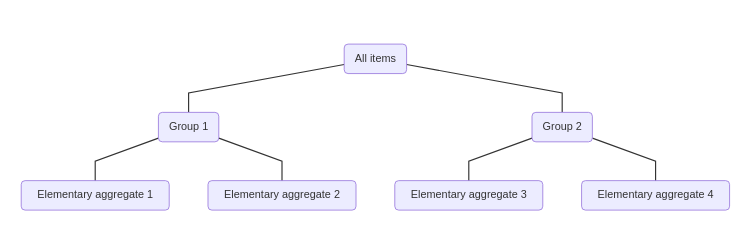
\includegraphics{img/plot1.png}

Une structure hiérarchique ne pose pas de problème particulier pour créer un indice de prix --- l'une des formules de numéro d'index de la section précédente peut toujours être utilisée pour agréger les prix relatifs des biens et services dans chaque groupe de la hiérarchie à produire une collection d'indices de prix pour chaque niveau de la hiérarchie. Le calcul de l'indice doit simplement être répété pour chaque groupe de biens et services dans la structure d'agrégation. Il s'agit de l'approche directe pour calculer un indice de prix avec une structure hiérarchique.

Cependant, avoir une structure hiérarchique suggère que le calcul peut être simplifié avec une procédure en deux étapes. Dans la première étape, les prix relatifs sont combinés au niveau d'agrégation le plus bas en utilisant l'une des formules de numéro d'index de la section précédente. Cela donne une collection d'indices de prix appelés indices élémentaires (ou élémentaires). Ces indices de prix donnent l'évolution des prix dans le temps pour de petits groupes de biens et services relativement homogènes appelés agrégats élémentaires qui constituent la base d'un indice de prix. Une fois les indices élémentaires calculés, les indices des niveaux d'agrégation supérieurs sont calculés en combinant les indices élémentaires à l'aide de pondérations. Ces pondérations fournissent une mesure de l'importance économique des biens et services dans chaque agrégat élémentaire afin de combiner les indices élémentaires pour former un indice de niveau supérieur. Si l'indice cible est un indice arithmétique, alors les agrégats élémentaires doivent être combinés avec une moyenne arithmétique pondérée; sinon, si un indice géométrique est l'indice cible, une moyenne géométrique pondérée doit être utilisée. Autrement dit, chaque agrégat élémentaire est traité comme un bien unique, les indices élémentaires étant les prix apparentés pour ces produits, et cette information est introduite dans une formule de nombre d'indice pour produire un indice de niveau supérieur.

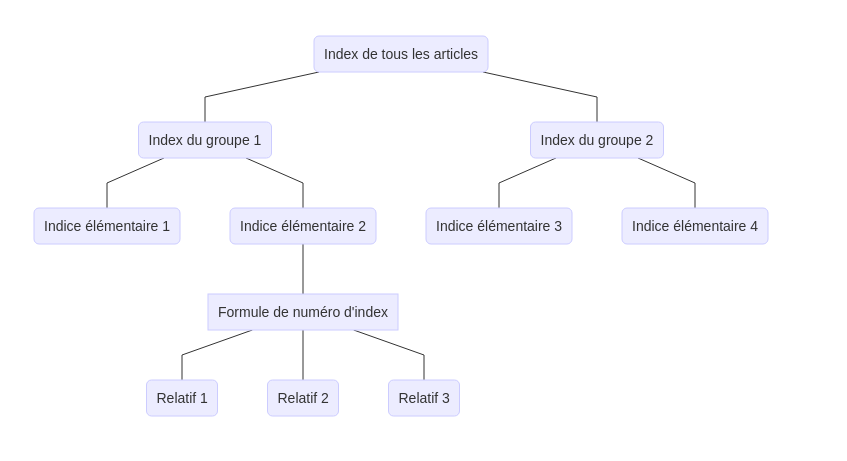
\includegraphics{img/plot2.png}

Étant donné qu'il existe deux façons de calculer un indice de prix avec une structure hiérarchique, le calcul direct donne-t-il le même résultat que le calcul en deux étapes? La réponse est oui pour un indice arithmétique ou géométrique, à condition que les poids utilisés pour agréger les agrégats élémentaires soient formés en utilisant les poids sous-jacents pour l'indice cible. Par exemple, si l'objectif est de calculer un indice de Laspeyres, le poids d'un agrégat élémentaire devrait être la part des dépenses / revenus pour les biens de cet agrégat élémentaire au cours de la période 0. Comme les indices géométriques et arithmétiques sont calculés en tant que moyennes pondérées, il ne devrait pas être surprenant qu'un indice puisse être calculé en regroupant d'abord les parents de prix, en calculant les moyennes au niveau du groupe, puis en faisant la moyenne des moyennes au niveau du groupe pour former une moyenne globale. Par conséquent, ces indices seraient cohérents dans l'agrégation, bien que toutes les formules de nombre d'indices ne soient pas cohérentes dans l'agrégation. Par exemple, l'indice de Fisher n'est pas cohérent dans l'agrégation, et l'utilisation de la procédure en deux étapes pour le calculer donnera une réponse différente de celle du calcul direct.

Il est facile de montrer que tout indice arithmétique est cohérent en agrégation (le raisonnement pour le cas géométrique est presque identique). Supposons que les marchandises soient partitionnées en \(k = 1, \ldots, m\) catégories distinctes et mutuellement exclusives --- c'est-à-dire qu'il y a \(m\) agrégats élémentaires. Si la catégorie \(k\) contient \(n_{k}\) biens, alors l'index arithmétique de cette catégorie est

\begin{align*}
I_{k}^{A} = \sum_{i = 1}^{n_k} \frac{\omega_{ik}}{\sum_{j = 1}^{n_k} \omega_{jk}} \frac{p_{ik1}}{p_{ik0}},
\end{align*}

où \(p_{ik1} / p_{ik0}\) est le prix relatif du bien \(i\) dans la catégorie \(k\) et \(\omega_{ik}\) est le poids du bien \(i\) dans la catégorie \(k\). Ces indices \(m\) peuvent maintenant être agrégés ensemble pour former un indice global en prenant une moyenne pondérée de chaque indice, avec des pondérations données par \(\omega_{k} = \sum_{j = 1}^{n_k} \omega_{jk}\), de sorte que

\begin{align*}
I^{A} &= \sum_{k = 1}^{m} \omega_k I_{k}^{A} \\
&= \sum_{k = 1}^{m} \omega_k \sum_{i = 1}^{n_k} \frac{\omega_{ik}}{\sum_{j = 1}^{n_k} \omega_{jk}} \frac{p_{ik1}}{p_{ik0}} \\
&= \sum_{k = 1}^{m} \sum_{i = 1}^{n_k} \omega_{ik} \frac{p_{ik1}}{p_{ik0}}.
\end{align*}

Mais c'est exactement la même chose que si l'indice arithmétique avait été calculé en regroupant tous les parents de prix et en calculant directement l'indice, plutôt que de les diviser en groupes et de calculer l'indice en deux étapes.

Un avantage du calcul en deux étapes par rapport au calcul direct est que la formule d'indice utilisée pour calculer les indices élémentaires peut différer de la formule d'indice utilisée à des niveaux d'agrégation plus élevés. Cela peut sembler étrange de vouloir le faire, mais il existe un certain nombre de raisons théoriques et pratiques subtiles pour lesquelles une formule d'indice différente serait utilisée pour les indices élémentaires. Dans la plupart des applications, les indices élémentaires sont calculés à l'aide d'un indice de Jevons, en partie parce que des informations détaillées sur les quantités achetées ou vendues peuvent être difficiles à obtenir à des niveaux d'agrégation très faibles. Des niveaux plus élevés sont ensuite calculés comme un indice arithmétique, généralement un indice de Young ou Lowe.

\hypertarget{factorisation-dun-index}{%
\subsection{Factorisation d'un index}\label{factorisation-dun-index}}

Lorsqu'il est calculé sur plusieurs périodes, un indice des prix donne une mesure de la variation des prix dans le temps par rapport à une période de base fixe. Le calcul d'un indice de prix sur de nombreuses périodes ne pose pas de nouveaux défis --- une fois qu'une période de base est sélectionnée, l'une des formules de nombre d'index dans la section précédente peut être directement appliquée pour produire un indice qui évolue au fil du temps en formant simplement des parents de prix qui calculez toujours la variation du prix par rapport à la période de base. Par exemple, la série d'indices géométriques calculés sur les périodes 0, 1 et 2, avec la période 0 comme période de base, est

\begin{align*}
1, \prod_{i = 1}^{n} \left (\frac{p_{i1}}{p_{i0}} \right)^{\omega_{i}}, \prod_{i = 1}^{n} \left (\frac{p_{i2}}{p_{i0}} \right)^{\omega_{i}}.
\end{align*}

Ainsi, la valeur de l'indice de la période 1 donne la variation des prix entre la période 1 et la période 0, et l'indice de la période 2 donne la variation des prix entre la période 2 et la période 0. La valeur de la période 0 est 1 car le rapport des prix de la période 0 à la période 0 prix est toujours 1.

La plupart des indices de prix sont calculés fréquemment --- généralement mensuellement ou trimestriellement --- et il est utile de pouvoir calculer un indice de prix en utilisant uniquement la valeur d'indice de la période précédente et les prix relatifs les plus récents pour chaque bien couvert par l'indice.\^{} {[}L'une des raisons est que cela peut faciliter l'échantillonnage des informations sur les prix, car les mêmes unités n'ont pas besoin d'être échantillonnées à la fois pour la période actuelle et la période de base.{]} C'est-à-dire qu'il est utile de pouvoir factoriser un indice en deux termes : la valeur de l'indice de la période précédente et un indice qui dépend uniquement des prix de la période en cours et des prix de la période précédente. Une telle factorisation permet de calculer un indice période par période et évite d'avoir à conserver les données de prix pendant la période de base pendant la durée de vie d'un indice. Ceci est pratiquement significatif, car cela signifie qu'un indice peut toujours être produit même si les données de prix de la période de base sont perdues.

La factorisation d'un indice géométrique est triviale; pour un ensemble de poids donné, l'index géométrique qui va de la période 0 à la période \(t\) peut toujours être écrit comme le produit de l'index géométrique qui va de la période 0 à la période \(k\) et de l'index géométrique qui va de la période \(k\) à la période \(t\). C'est,

\begin{align*}
I^{G}(0, t) & = \prod_{i = 1}^{n} \left (\frac{p_{it}}{p_{i0}} \right)^{\omega_i} \\
& = \prod_{i = 1}^{n} \left (\frac{p_{ik}}{p_{i0}} \right)^{\omega_i} \times \prod_{i = 1}^{n } \left (\frac{p_{it}}{p_{ik}} \right)^{\omega_i} \\
& = I^{G}(0, k) \times I^{G}(k, t).
\end{align*}

Cela devrait être profondément intuitif. Si les prix ont augmenté de 20\% entre la période 0 et la période \(k\), puis augmentent de 10\% supplémentaires entre la période \(k\) et la période \(t\), l'augmentation totale du prix de la période 0 à la période \(t\) est de 32\%. Cela revient à multiplier une valeur d'index de 1,2 par une valeur d'index de 1,1, car le résultat est 1,32.

La factorisation d'un indice arithmétique est légèrement plus complexe, car elle nécessite de modifier les pondérations utilisées pour agréger les prix relatifs. L'index arithmétique qui s'étend de la période 0 à la période \(t\) peut être écrit comme

\begin{align*}
I^{A}(0, t) & = \sum_{i = 1}^{n} \omega_{i} \frac{p_{it}}{p_{i0}} \\
& = I^{A}(0, k) \times \sum_{i = 1}^{n} \tilde{\omega}_{i} \frac{p_{it}}{p_{ik}},
\end{align*}

où

\begin{align*}
\tilde{\omega}_{i} = \frac{\omega_{i} \frac{p_{ik}}{p_{i0}}}{I^{A}(0, k)}.
\end{align*}

Contrairement à l'index géométrique, la factorisation d'un index arithmétique nécessite de changer les pondérations de l'index allant de la période \(k\) à \(t\). Parfois, cela s'appelle le prix mettant à jour les poids, mais cette terminologie est utilisée de manière incohérente. Malgré cette ride, cependant, l'idée de base est la même que dans le cas géométrique --- un indice arithmétique peut toujours être décomposé en deux indices arithmétiques.

Intuitivement, la factorisation d'un indice bricole simplement la valeur de l'indice dans la période de base afin qu'il puisse continuer à partir d'une valeur précédente sans avoir besoin d'être recalculé dès le départ. Plutôt que de commencer l'indice à la valeur 1 de la période \(k\), il part de la valeur de l'indice de la période \(k\), s'appuyant essentiellement sur la variation cumulative des prix jusqu'à ce moment-là.

\hypertarget{rebasing}{%
\subsection{Rebasing}\label{rebasing}}

La période de base est un moment important pour un indice des prix, car elle donne le point de référence fixe par rapport auquel les variations de prix sont mesurées. Cependant, le fait de devoir choisir une période de base introduit un problème potentiel: ce qui fonctionne comme période de base pour une utilisation d'un indice de prix peut ne pas fonctionner pour une autre. Heureusement, le choix de la période de base n'a pas beaucoup d'impact sur le contenu économique d'un indice des prix --- dans la plupart des cas, une nouvelle période de base peut être choisie pour un indice sans avoir à recalculer la série d'indices entière.

Pour un indice géométrique, le choix de la période de base n'a aucun impact sur le contenu économique d'un indice de prix --- la variation de prix entre deux périodes quelconques est la même quelle que soit la période de base. La période de base standardise simplement l'indice à un niveau particulier. Cela peut être vu en rappelant qu'un indice géométrique peut toujours être factorisé en deux indices géométriques. Étant donné une série d'indices avec la période 0 comme période de base, la valeur de l'indice dans la période \(t\) avec la période \(k\) comme période de base peut toujours être trouvée en divisant simplement la valeur de l'indice dans la période \(t\) par la valeur de l'indice dans la période \(k\)

\begin{align*}
I^{G}(k, t) & = \prod_{i = 1}^{n} \left (\frac{p_{it}}{p_{ik}} \right)^{\omega_{i} } \\
& = \frac{\prod_{i = 1}^{n} \left (\frac{p_{it}}{p_{i0}} \right)^{\omega_{i}}}{\prod_{i = 1}^{n} \left (\frac{p_{ik}}{p_{i0}} \right)^{\omega_{i}}} \\
& = \frac{I^{G}(0, t)}{I^{G}(0, k)}.
\end{align*}

Par conséquent, la division de la série d'indices par la valeur d'index de la période \(k\) produit une série d'indices qui est la même que si la période \(k\) était initialement choisie comme période de base. C'est ce que l'on appelle le rebasage d'un indice et cela signifie qu'un changement de prix entre deux périodes peut être calculé en mettant simplement à l'échelle l'indice des prix. Cela explique également pourquoi la période de base obtient une valeur dans la série d'indices, sinon la série d'indices se rétrécirait chaque fois que l'indice est rebasé.

Le graphique ci-dessous donne un exemple de la façon dont le rebasage modifie la série chronologique. L'indice avec une période de base de décembre est simplement l'indice avec une période de base de janvier divisé par la valeur de l'indice en décembre (105). Cela déplace simplement l'indice avec janvier comme période de base vers le bas, et l'écrase un peu, mais ne change pas la forme relative de la série chronologique.

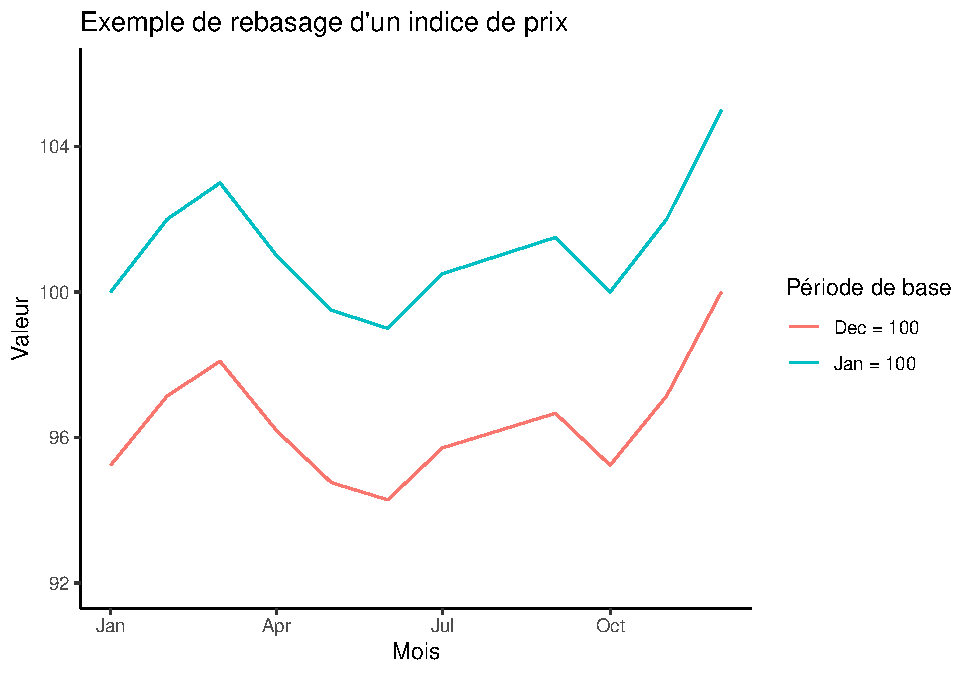
\includegraphics{cours-indices-des-prix_files/figure-latex/unnamed-chunk-6-1.pdf}

La recadrage est plus complexe pour un index arithmétique. Bien qu'il fonctionne pour un indice de Lowe et Dutot de la même manière qu'un indice géométrique, en général, le rebasage d'un indice arithmétique modifie les pondérations utilisées pour la moyenne des prix relatifs en raison de la façon dont un indice arithmétique est factorisé. L'indice rebasé est toujours un indice arithmétique, mais les poids ne sont plus corrects. Par exemple, le rebasage d'un indice de Laspeyres modifie les pondérations afin qu'elles ne soient plus les parts de dépenses de la période de base --- l'indice est toujours un indice arithmétique (un indice de Lowe), mais des produits qui ont connu une augmentation de prix plus importante depuis le la période de base recevra plus de poids dans le calcul de l'indice. En pratique, cependant, cette ride théorique est généralement ignorée, et un indice de prix arithmétique est rebasé en divisant simplement la série d'indices entière par la valeur de l'indice dans la nouvelle période de base.

\hypertarget{chauxeenage}{%
\subsection{Chaînage}\label{chauxeenage}}

Les pondérations d'un indice donnent idéalement une mesure de l'importance économique des biens qui le composent, de sorte que les prix apparentés pour les biens et services de plus grande importance économique ont une plus grande influence sur l'évolution globale des prix entre les périodes. Dans l'application, les poids sont souvent réutilisés au fil du temps, car il est coûteux et long de mettre à jour en permanence les poids. Le maintien des mêmes poids période après période, cependant, signifie que les poids finiront par devenir obsolètes et pourraient ne pas saisir les changements dans l'importance économique de certains biens. Le chaînage d'un index permet de mettre à jour les pondérations d'un index et d'ajouter de nouvelles valeurs d'index aux séries d'index calculées avec les anciennes pondérations, sans avoir à réviser les anciennes séries d'index. Le chaînage peut également être utilisé pour modifier la composition des biens et services couverts par un indice des prix, et cela peut changer à mesure que de nouveaux biens sont introduits sur un marché et que des biens anciens disparaissent.

L'idée derrière le chaînage est la même que celle de la factorisation d'un index --- divisez un index en deux morceaux qui peuvent être collés ensemble à une période de chevauchement commune. La différence est que, bien que la factorisation d'un indice est simplement une astuce d'algèbre, le chaînage d'un index est une solution pratique pour produire un index avec une série chronologique plus longue, plutôt que de redémarrer l'index dans la période où les pondérations changent. Dans les deux cas, l'idée est de modifier la valeur de la période de base d'un indice pour refléter la variation cumulative des prix jusqu'à ce moment-là.

Les étapes de chaînage de tout type d'index sont les mêmes, alors considérez un index arithmétique allant de la période 0 à la période \(t\), et supposez que les pondérations de cet indice changent au cours d'une période \(k\). Cela pourrait être dû au fait que les pondérations précédentes sont devenues suffisamment obsolètes pour être modifiées, ou que les biens et services auxquels l'indice s'applique ont changé. Quelle que soit la raison, cela donne lieu à deux indices, l'un allant de la période 0 à la période \(k\), utilisant des pondérations de la période 0

\begin{align*}
I^{A}(0, k) = \sum_{i = 1}^{n} \omega_{i0} \frac{p_{ik}}{p_{i0}},
\end{align*}

et un autre allant de la période \(k\) à la période \(t\) en utilisant les pondérations period-\(k\)

\begin{align*}
I^{A}(k, t) = \sum_{i = 1}^{m} \omega_{ik} \frac{p_{it}}{p_{ik}}.
\end{align*}

L'indice chaîné multiplie simplement ces deux indices ensemble, de sorte que

\begin{align*}
I^{A}(0, t) = \sum_{i = 1}^{n} \omega_{i0} \frac{p_{ik}}{p_{i0}} \times \sum_{i = 1}^{m} \omega_{ik} \frac{p_{it}}{p_{ik}}.
\end{align*}

Le graphique ci-dessous donne un exemple de ce à quoi ressemble un indice chaîné.

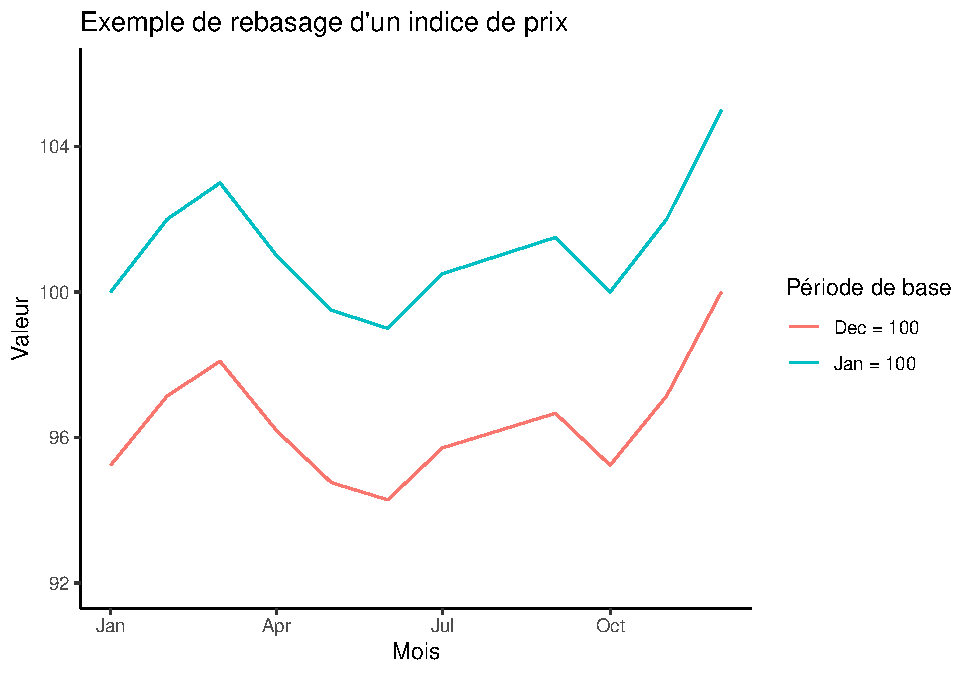
\includegraphics{cours-indices-des-prix_files/figure-latex/unnamed-chunk-7-1.pdf}

La partie importante d'un indice chaîné est la période de chevauchement \(k\) lorsque les pondérations changent et les prix de la période \(k\) sont utilisés avec deux ensembles de pondérations. S'il n'y a pas de période de chevauchement, alors l'index ne peut pas être enchaîné. Chaque indice peut être considéré comme un maillon de la chaîne, donnant le mouvement des prix pour cette partie du temps, et la période de chevauchement est l'endroit où les maillons se rencontrent.

\hypertarget{exemple-avec-r-1}{%
\subsection{Exemple avec R}\label{exemple-avec-r-1}}

Il est utile de terminer cette section du cours avec quelques exemples dans R. Le premier exemple montre qu'un indice géométrique est cohérent dans l'agrégation. Le calcul de l'indice en deux étapes donne la même réponse que le calcul direct.

\begin{Shaded}
\begin{Highlighting}[]
\CommentTok{# Apportez dans la bibliothèque ppd}
\KeywordTok{library}\NormalTok{(ppd)}

\CommentTok{# Faites des prix apparentés}
\NormalTok{dat <-}\StringTok{ }\KeywordTok{data.frame}\NormalTok{(}\DataTypeTok{relatives =} \KeywordTok{c}\NormalTok{(}\FloatTok{1.1}\NormalTok{, }\FloatTok{1.2}\NormalTok{, }\FloatTok{0.9}\NormalTok{, }\FloatTok{1.1}\NormalTok{),}
                  \DataTypeTok{weight =} \KeywordTok{c}\NormalTok{(}\FloatTok{0.25}\NormalTok{, }\FloatTok{0.3}\NormalTok{, }\FloatTok{0.3}\NormalTok{, }\FloatTok{0.15}\NormalTok{),}
                  \DataTypeTok{group =}\NormalTok{ letters[}\KeywordTok{c}\NormalTok{(}\DecValTok{1}\NormalTok{, }\DecValTok{1}\NormalTok{, }\DecValTok{2}\NormalTok{, }\DecValTok{2}\NormalTok{)]}
\NormalTok{)}
\NormalTok{dat}
\end{Highlighting}
\end{Shaded}

\begin{verbatim}
##   relatives weight group
## 1       1.1   0.25     a
## 2       1.2   0.30     a
## 3       0.9   0.30     b
## 4       1.1   0.15     b
\end{verbatim}

\begin{Shaded}
\begin{Highlighting}[]
\CommentTok{# Calculer l'indice géométrique pour les parents des groupes a et b}
\NormalTok{index_ab <-}\StringTok{ }\KeywordTok{sapply}\NormalTok{(}\KeywordTok{split}\NormalTok{(dat, dat}\OperatorTok{$}\NormalTok{group), }
                   \ControlFlowTok{function}\NormalTok{(x) }\KeywordTok{geomean}\NormalTok{(x}\OperatorTok{$}\NormalTok{relatives, x}\OperatorTok{$}\NormalTok{weight) }\OperatorTok{*}\StringTok{ }\DecValTok{100}
\NormalTok{                   )}
\NormalTok{index_ab}
\end{Highlighting}
\end{Shaded}

\begin{verbatim}
##         a         b 
## 115.34655  96.22603
\end{verbatim}

\begin{Shaded}
\begin{Highlighting}[]
\CommentTok{# Indices agrégés de niveau inférieur}
\NormalTok{index_top <-}\StringTok{ }\KeywordTok{geomean}\NormalTok{(index_ab, }\KeywordTok{tapply}\NormalTok{(dat}\OperatorTok{$}\NormalTok{weight, dat}\OperatorTok{$}\NormalTok{group, sum))}
\NormalTok{index_top}
\end{Highlighting}
\end{Shaded}

\begin{verbatim}
## [1] 106.3125
\end{verbatim}

\begin{Shaded}
\begin{Highlighting}[]
\CommentTok{# Identique au calcul direct}
\KeywordTok{geomean}\NormalTok{(dat}\OperatorTok{$}\NormalTok{relatives, dat}\OperatorTok{$}\NormalTok{weight) }\OperatorTok{*}\StringTok{ }\DecValTok{100}
\end{Highlighting}
\end{Shaded}

\begin{verbatim}
## [1] 106.3125
\end{verbatim}

Le deuxième exemple montre comment rebaser un indice de prix --- divisez simplement la série d'indices par la valeur de l'indice dans la nouvelle période de base.

\begin{Shaded}
\begin{Highlighting}[]
\CommentTok{# Faire un index sur 12 périodes avec période 0 = 100}
\NormalTok{index <-}\StringTok{ }\KeywordTok{data.frame}\NormalTok{(}\DataTypeTok{period =} \DecValTok{0}\OperatorTok{:}\DecValTok{11}\NormalTok{, }\DataTypeTok{value =} \KeywordTok{c}\NormalTok{(}\DecValTok{100}\NormalTok{, }\KeywordTok{sample}\NormalTok{(}\DecValTok{90}\OperatorTok{:}\DecValTok{130}\NormalTok{, }\DecValTok{11}\NormalTok{)))}
\NormalTok{index}
\end{Highlighting}
\end{Shaded}

\begin{verbatim}
##    period value
## 1       0   100
## 2       1   116
## 3       2   111
## 4       3   113
## 5       4   126
## 6       5   124
## 7       6    93
## 8       7   115
## 9       8   123
## 10      9    94
## 11     10    90
## 12     11    96
\end{verbatim}

\begin{Shaded}
\begin{Highlighting}[]
\CommentTok{# Rebase l'indice pour que la période 6 = 100}
\KeywordTok{transform}\NormalTok{(index, }\DataTypeTok{value =}\NormalTok{ value }\OperatorTok{/}\StringTok{ }\NormalTok{value[period }\OperatorTok{==}\StringTok{ }\DecValTok{6}\NormalTok{] }\OperatorTok{*}\StringTok{ }\DecValTok{100}\NormalTok{)}
\end{Highlighting}
\end{Shaded}

\begin{verbatim}
##    period     value
## 1       0 107.52688
## 2       1 124.73118
## 3       2 119.35484
## 4       3 121.50538
## 5       4 135.48387
## 6       5 133.33333
## 7       6 100.00000
## 8       7 123.65591
## 9       8 132.25806
## 10      9 101.07527
## 11     10  96.77419
## 12     11 103.22581
\end{verbatim}

\hypertarget{affectation}{%
\section{Affectation}\label{affectation}}

Les réponses à ces questions proviennent à la fois du contenu du cours et des lectures. Chaque question vaut un point, pour un total de 20 points. La réussite de ce module nécessite au moins 65\% (13 sur 20 correct). Envoyez vos réponses par e-mail à l'instructeur du cours lorsque vous avez terminé.

\textbf{Question 1} Vrai ou faux: l'indice Jevons est toujours inférieur ou égal à l'indice Laspeyres.

\textbf{Question 2} Pourquoi l'indice Laspeyres est-il toujours plus grand que l'indice Paasche?

\begin{enumerate}
\def\labelenumi{\alph{enumi})}
\item
  Biais de substitution.
\item
  Les quantités sont mesurées moins précisément dans l'indice de Paasche, de sorte que la variation d'échantillonnage est
  plus grand.
\item
  Les tendances saisonnières de la consommation sont surestimées dans l'indice de Laspeyres.
\item
  L'indice Laspeyres peut être plus petit que l'indice Paasche.
\item
  Aucune de ces réponses.
\end{enumerate}

\textbf{Question 3} Lesquels des éléments suivants sont des utilisations d'un indice des prix à la production?

\begin{enumerate}
\def\labelenumi{\alph{enumi})}
\item
  Indicateur des tendances inflationnistes des intrants des producteurs.
\item
  Déflateur des comptes nationaux.
\item
  Indicateur des tendances inflationnistes pour les biens et services de consommation.
\item
  Marge d'ajustement cyclique de la balance des paiements.
\item
  a et b.
\item
  a, b et d.
\item
  Tout ce qui précède.
\end{enumerate}

\textbf{Question 4} Vrai ou faux: l'indice Jevons est toujours inférieur ou égal à l'indice Carli.

\textbf{Question 5} Vrai ou faux: un indice des prix à la consommation donne une mesure du niveau de prix global auquel sont confrontés les consommateurs.

\textbf{Question 6} Lesquels des éléments suivants sont des utilisations d'un indice des prix à la consommation?

\begin{enumerate}
\def\labelenumi{\alph{enumi})}
\item
  Indicateur des tendances inflationnistes pour les biens et services de consommation.
\item
  Déflateur des comptes nationaux.
\item
  Indicateur des tendances inflationnistes de la production des producteurs.
\item
  Indexation des salaires.
\item
  a et b.
\item
  a, b et d.
\item
  Tout ce qui précède.
\end{enumerate}

\textbf{Question 7} Quels sont les trois types d'indices des prix à la production?

\begin{enumerate}
\def\labelenumi{\alph{enumi})}
\item
  Prix d'entrée, prix de sortie, prix de transfert.
\item
  Prix d'entrée, valeur ajoutée, prix à la consommation.
\item
  Prix de sortie, prix d'entrée, valeur ajoutée.
\item
  Prix d'entrée, prix de sortie, valeur ajoutée.
\item
  Aucune de ces réponses.
\end{enumerate}

\textbf{Question 8} Qu'est-ce qu'un indice élémentaire?

\begin{enumerate}
\def\labelenumi{\alph{enumi})}
\item
  Le prix des intrants bruts pour une entreprise.
\item
  Les indices de prix pour le niveau le plus bas d'une hiérarchie.
\item
  Les prix individuels des répondants.
\item
  La valeur des biens et services achetés au niveau le plus bas d'une hiérarchie.
\item
  Aucune de ces réponses.
\end{enumerate}

\textbf{Question 9} Quel est le classement habituel des indices Fisher, Laspeyres, Lowe et Paasche en fonction de leur ampleur (c'est-à-dire que la demande diminue lorsque les prix augmentent)?

\begin{enumerate}
\def\labelenumi{\alph{enumi})}
\item
  Laspeyres ≥ Lowe ≥ Paasche ≥ Fisher.
\item
  Lowe ≥ Laspeyres ≥ Fisher ≥ Paasche.
\item
  Paasche ≥ Fisher ≥ Laspeyres ≥ Lowe.
\item
  Fisher ≥ Lowe ≥ Laspeyres ≥ Paasche.
\item
  Aucune de ces réponses.
\end{enumerate}

\textbf{Question 10} Vrai ou faux: les pondérations pour l'agrégation d'un indice doivent être basées sur l'échantillon de prix utilisé pour calculer les agrégats élémentaires.

\textbf{Question 11} Vrai ou faux: un indice de Fisher est considéré comme le meilleur type d'index car il est très opportun à produire.

\textbf{Question 12} Lesquels des éléments suivants sont des indices symétriques?

\begin{enumerate}
\def\labelenumi{\alph{enumi})}
\item
  Fisher, Laspeyres, Paasche.
\item
  Jevons, Lowe.
\item
  Fisher, Törnqvist.
\item
  Jeune.
\item
  Aucune de ces réponses.
\end{enumerate}

\textbf{Question 13} Vrai ou faux: les indices Dutot et Jevons sont tous deux transitifs.

\textbf{Question 14} Les pondérations pour un indice des prix à la production devraient toujours être basées sur.

\begin{enumerate}
\def\labelenumi{\alph{enumi})}
\item
  Parts des revenus.
\item
  Part des dépenses.
\item
  Valeur ajoutée.
\item
  Parts des revenus actuels et futurs.
\item
  Aucune de ces réponses.
\end{enumerate}

\textbf{Question 15} Vrai ou faux: tous les indices de prix peuvent être classés comme arithmétiques, géométriques ou harmoniques.

\textbf{Question 16} Les pondérations pour un indice des prix à la consommation peuvent provenir de quelles sources.

\begin{enumerate}
\def\labelenumi{\alph{enumi})}
\item
  Données du scanner.
\item
  Enquête sur les dépenses de consommation.
\item
  Comptes nationaux.
\item
  Recensement de la population.
\item
  a et b.
\item
  Tout ce qui précède.
\item
  Aucune de ces réponses.
\end{enumerate}

\textbf{Question 17} Un indice a une valeur de 90 en janvier et une valeur de 130 en mai. Quelle est la valeur de l'indice en mai si janvier est défini comme période de base?

\begin{enumerate}
\def\labelenumi{\alph{enumi})}
\item
  90,0.
\item
  100,0.
\item
  140,0.
\item
  144,4.
\item
  130,0.
\end{enumerate}

\textbf{Question 18} Vrai ou faux: l'indice de Fisher est cohérent dans l'agrégation.

\textbf{Question 19} Un indice des prix a une valeur de 80 en mars et 90 en septembre. Quel est le pourcentage de variation des prix entre mars et septembre?

\begin{enumerate}
\def\labelenumi{\alph{enumi})}
\item
  10\%.
\item
  12,5\%.
\item
  -11\%.
\item
  Aucune de ces réponses.
\item
  Il est impossible de savoir sans connaître la période de base.
\end{enumerate}

\textbf{Question 20} Vous essayez de faire un index pour les widgets bleus et rouges. Le prix relatif des widgets rouges est de 1,2 et le prix relatif des widgets bleus est de 0,9. La part des dépenses consacrées aux widgets rouges est de 0,3 au cours de la période de base et de 0,25 au cours de la période en cours; la part des dépenses pour les widgets bleus est de 0,7 pour la période de base et de 0,75 pour la période en cours. Quelle est la valeur de l'indice géométrique de Laspeyres?

\begin{enumerate}
\def\labelenumi{\alph{enumi})}
\item
  98,1.
\item
  96,7.
\item
  97,4.
\item
  99,0.
\item
  97,5.
\end{enumerate}

\hypertarget{part-thuxe9orie-de-lindice-des-prix}{%
\part{Théorie de l'indice des prix}\label{part-thuxe9orie-de-lindice-des-prix}}

\hypertarget{programme-1}{%
\section{Programme}\label{programme-1}}

Pourquoi certaines formules de numéro d'indice sont-elles utilisées pour calculer un indice de prix? Répondre à cette question nécessite une théorie des indices de prix qui peut être utilisée pour évaluer les propriétés d'un indice de prix et déterminer si un numéro d'indice est meilleur qu'un autre.

L'objectif de ce module est de fournir les fondements théoriques d'un indice des prix, avec un accent particulier sur la motivation des formules d'indice-nombre qui sont utilisées dans la pratique. À la fin du module, une personne devrait:

\begin{enumerate}
\def\labelenumi{\arabic{enumi}.}
\item
  Familiarisez-vous avec les trois approches théoriques pour développer un indice des prix.
\item
  Savoir comment les trois approches peuvent être utilisées pour motiver les numéros d'index couramment utilisés.
\end{enumerate}

Ce module est utile à la fois pour les utilisateurs et les compilateurs d'indices de prix avec une compréhension de base de la façon de construire un indice de prix, et qui aimerait mieux comprendre pourquoi des formules d'indice-nombre particulières sont utilisées.

Ce module se compose de lectures autodirigées, accompagnées d'un devoir. Au total, environ 10 à 15 heures devraient être consacrées à ce module.

Prérequis: Introduction aux indices de prix, au moins un cours de micro-théorie intermédiaire et au moins un cours d'introduction aux probabilités et aux statistiques. Un cours avancé de micro-théorie est utile.

L'évaluation de ce module est basée sur une tâche composée de 20 questions à choix multiples / vrai-faux qui s'appuient sur du matériel dans le contenu du cours et les lectures. La collaboration sur la mission est la bienvenue, mais chaque personne doit soumettre son propre travail unique. La réussite de ce module nécessite au moins 65\% sur l'affectation.

Les lectures de ce module proviennent des chapitres 15 à 18 du manuel PPI (ILO et al. 2004b) et / ou du manuel CPI (ILO et al. 2004a), publié par le FMI (disponible gratuitement sur leur site Internet), ainsi que de la revue des prix. théorie de l'indice par Balk (1995).

Veuillez envoyer un e-mail à l'instructeur du cours si vous avez des questions ou si vous avez besoin d'aide concernant le matériel ou le devoir du cours.

\hypertarget{introduction}{%
\section{Introduction}\label{introduction}}

Il existe trois grandes approches pour motiver les formules d'indice des prix qui sont utilisées dans la pratique par les organismes statistiques: l'approche axiomatique, l'approche économique et l'approche stochastique. Chaque approche est utile en soi, et les trois donnent des perspectives et des compréhensions différentes pour les diverses formules de nombre d'indices qui sont utilisées pour construire des indices de prix. Ensemble, ces différentes approches constituent une théorie des indices de prix.

Chacune des trois approches peut être considérée comme répondant à une question différente sur la façon de construire un indice des prix. L'approche axiomatique tente de répondre à la question ``Comment combiner les informations d'une collection de prix et de quantités pour satisfaire certaines propriétés?'' Il s'agit essentiellement d'une approche théorique définie sur la meilleure façon de construire un numéro d'index. En revanche, l'approche économique tente de répondre à la question ``Que doit mesurer un indice des prix?'' Le but de l'approche économique est d'utiliser le mécanisme de la théorie microéconomique pour définir un indice des prix afin de mesurer l'expérience d'un changement de prix pour les consommateurs et les producteurs. L'approche stochastique est plus pragmatique dans sa portée et tente de répondre à la question ``Comment les informations sur les prix peuvent-elles être utilisées pour prédire au mieux un changement de prix pour un bien ou un service?'' Il s'agit essentiellement d'une question sur la meilleure façon de gonfler et de dégonfler les prix au fil du temps.

Cette partie du cours donne une introduction pratique à chacune des trois approches, en se concentrant sur la façon dont elles peuvent être utilisées pour motiver la manière dont les indices de prix sont construits dans la pratique. Bien qu'il ait une orientation plus pratique, cependant, ce matériel est toujours concerné par une théorie qui peut être assez technique. Plutôt que de se concentrer sur les détails techniques (dont ils sont nombreux), cette partie du cours donne un aperçu suffisant de la machinerie technique pour montrer ce qui se passe, tout en fournissant l'intuition économique et les idées générales de la théorie.

\hypertarget{lapproche-axiomatique}{%
\section{L'approche axiomatique}\label{lapproche-axiomatique}}

Un indice des prix combine des informations sur les prix et les quantités à deux moments afin de produire un rapport de prix entre ces moments. À moins qu'il n'y ait qu'un seul prix à chaque moment, cependant, il n'y a pas de moyen unique de combiner les prix au fil du temps --- il existe une infinité de formules de numéros d'index possibles qui peuvent être utilisées pour calculer un indice de prix. Cet embarras des richesses n'est pas souhaitable, car il introduit un choix considérable sur la manière de mesurer un changement de prix. L'approche axiomatique tente de résoudre ce problème en considérant une classe générale d'indices de prix et en trouvant quels membres de cette classe satisfont certaines propriétés intuitives ou raisonnables qu'un indice de prix devrait satisfaire. Cela équivaut à faire une déclaration normative sur la façon dont un indice des prix devrait se comporter --- quels sont les axiomes fondamentaux qui définissent un indice des prix? L'idée est de commencer par une classe très large de formules d'indices possibles et de définir des axiomes pour réduire les formules d'indices qui ne se comportent pas comme un indice de prix.

Le résultat idéal de l'approche axiomatique est une formule d'indice unique et unique qui satisfait un ensemble minimal de conditions non controversées qu'un indice de prix devrait satisfaire. Cela signifierait qu'il n'y a qu'une seule formule d'indice qui devrait être utilisée pour créer un indice de prix. La réalité, cependant, est que des compromis doivent être faits, et le maintien de certaines conditions nécessite d'ignorer les autres. Par conséquent, une distinction est faite entre les axiomes --- déclarations fondamentales que tout indice de prix raisonnable devrait satisfaire --- et les tests, qui sont des propriétés souhaitables mais pas aussi fondamentales que les axiomes. Un petit ensemble d'axiomes clés est toujours conservé, tandis que les tests peuvent être mutuellement incohérents, et des choix doivent être faits quant aux tests qu'un index doit satisfaire en fonction de son objectif. Les axiomes peuvent être considérés comme le premier tamis à éliminer toutes les formules de nombre d'index déraisonnables, avec des tests agissant comme un second tamis pour affiner davantage ce qui reste.

Cette section du cours commence le voyage dans la théorie de l'indice des prix en donnant un bref aperçu de l'approche axiomatique de la théorie de l'indice des prix. Cela a été un domaine d'étude considérable, et par conséquent il y a beaucoup de matériel intéressant qui n'est pas couvert dans ce cours. Le lecteur intéressé peut consulter ILO et al. (2004a Chapitre 16) ou ILO et al. (2004b Chapter 16) pour plus de détails, ou Balk (2008).

📖 Balk (1995), ignorez la section 4 et l'annexe.

📖 Manuel PPI: Chapitre 1, section C.

\hypertarget{un-indice-de-prix-abstrait}{%
\subsection{Un indice de prix abstrait}\label{un-indice-de-prix-abstrait}}

Dans sa forme abstraite, un indice de prix est une fonction \(I\) qui prend quatre arguments --- prix période-0 \(p_{0}\), période-\(t\) prix \(p_{t}\), quantités période-0 \(q_{0}\) et period-\(t\) quantités \(q_{t}\), pour \(n\) biens et services distincts --- et renvoie une valeur unique. Il s'agit d'une règle qui transforme les informations sur les prix et les quantités à deux moments différents en un seul chiffre qui résume la variation des prix. Pour simplifier la notation, les prix et les quantités sont ici des vecteurs de prix et de quantités à un moment donné; par exemple, avec \(n\) biens et services distincts, les prix de la période 0 sont donnés par \(p_0 = (p_{10}, p_{20}, \ldots, p_{n0})\). Cette notation est utile, car un indice de prix est un moyen de distiller des informations pour de nombreux prix et quantités en une seule valeur; par exemple, avec 25 biens et services, l'indice des prix prend 100 pièces pour information (50 prix et 50 quantités) et la transforme en une seule information. Pour une collection particulière de prix et de quantités, la valeur de l'indice est donnée par \(I(p_{t}, p_{0}, q_{t}, q_{0})\).

La plupart des indices de prix peuvent être exprimés sous cette forme abstraite. Par exemple, un indice de Laspeyres est simplement

\begin{align*}
I(p_{t}, p_{0}, q_{t}, q_{0}) = \frac{\sum_{i = 1}^{n} p_{it} q_{i0}} {\sum_{i = 1}^{n} p_{i0} q_{i0}}.
\end{align*}

Les formules de numéros d'index qui n'utilisent pas d'informations sur les quantités ne nécessitent aucun traitement spécial --- la valeur de l'indice est juste indépendante des quantités vendues. Par exemple, l'indice Jevons est

\begin{align*}
I(p_{t}, p_{0}, q_{t}, q_{0}) = \prod_{i = 1}^{n} \left(\frac{p_{it}} {p_{i0} } \right)^{1 / n}.
\end{align*}

Bien que la plupart des formules d'indice correspondent à cette représentation abstraite, les indices de prix qui utilisent des informations dans une période autre que la période 0 ou la période \(t\), comme un indice Lowe ou Young, ne le font pas. C'est un point important, car l'approche axiomatique ignore implicitement ces types d'indices de prix dès le départ, plutôt que d'utiliser des axiomes pour évaluer leur caractère raisonnable en tant qu'indice de prix.

\hypertarget{les-axiomes}{%
\subsection{Les axiomes}\label{les-axiomes}}

Il existe cinq axiomes clés que tout indice de prix devrait satisfaire pour toutes les collections de prix et de quantités. Ces axiomes peuvent être considérés comme généralisant les propriétés du rapport des prix entre la période \(t\) et la période 0 pour un seul bien ou service à des environnements avec de nombreux biens et services.

\begin{enumerate}
\def\labelenumi{\arabic{enumi}.}
\item
  \textbf{Monotonie} \(I(p'_{t}, p_{0}, q_{t}, q_{0})> I(p_{t}, p_{0}, q_{t}, q_{0})\) if \(p'_{t} \geq p_{t}\) and \(p'_{t} \neq p_{t}\) et \(I(p_{t}, p'_{0}, q_{t}, q_{0}) <I(p_{t}, p_{0}, q_{t}, q_{0})\) if \(p'_{0} \geq p_{0 }\) et \(p'_{0} \neq p_{0}\).
\item
  \textbf{Homogénéité linéaire} \(I(cp_{t}, p_{0}, q_{t}, q_{0}) = cI(p_{t}, p_{0}, q_{t}, q_{0})\) pour tout \(c> 0\).
\item
  \textbf{Identité} \(I(p_{0}, p_{0}, q_{t}, q_{0}) = 1\).
\item
  \textbf{Homogénéité du degré zéro} \(I(cp_{t}, cp_{0}, q_{t}, q_{0}) = I(p_{t}, p_{0}, q_{t} , q_{0})\) pour tout \(c> 0\).
\item
  \textbf{Invariance dimensionnelle} Si \(A\) est une matrice diagonale de nombres positifs, alors \(I(Ap_{t}, Ap_{0}, A^{-1} q_{t}, A^{-1} q_{0}) = I(p_{t}, p_{0}, q_{t}, q_{0})\).
\end{enumerate}

Tous ces axiomes sont assez simples à comprendre d'après leur représentation mathématique, peut-être à l'exception de l'invariance dimensionnelle, et sont assez intuitifs. La monotonie signifie simplement qu'un indice de prix augmente dans les prix de la période \(t\) et diminue dans les prix de la période 0 --- les prix \(t\) de la période plus grande produisent des valeurs d'indice plus élevées et les prix de la période 0 plus grands produisent des valeurs d'indice plus petites. Cela semble être une condition nécessaire pour qu'un indice des prix puisse mesurer de manière significative l'inflation, car un indice qui ne satisfait pas à la monotonie peut diminuer lorsque les prix augmentent.

L'homogénéité linéaire est probablement la moins intuitive des axiomes, et dit que multiplier tous les prix de la période \(t\) par une constante équivaut à multiplier l'indice entier par une constante, de sorte qu'une augmentation proportionnelle des prix se traduit par une augmentation proportionnelle du indice. Pour voir pourquoi cela a du sens, considérons deux villes (A et B) qui ont toutes les mêmes prix dans la période 0. Si tous les prix dans la ville A augmentent de deux fois plus que les prix dans la ville B entre la période 0 et la période \(t\), les quantités achetées restant les mêmes dans les deux villes (car les prix relatifs sont les mêmes dans les deux villes), alors il est raisonnable de dire que les prix dans la ville A ont augmenté deux fois plus que dans la ville B.

L'axiome identitaire est simple et indique qu'un indice des prix ne montre pas de changement de prix si les prix ne changent pas. Comme l'axiome de monotonie, cela semble être une exigence nécessaire pour un indice des prix pour mesurer l'inflation; sinon, un indice des prix pourrait montrer une variation des prix lorsque les prix ne changent pas avec le temps.

L'homogénéité du degré zéro signifie que la multiplication de tous les prix par une constante n'a aucun impact sur un indice --- la devise dans laquelle les prix sont mesurés n'affecte pas la valeur d'un indice de prix. Une formule d'indice qui ne satisfait pas à l'homogénéité du degré zéro peut donner une mesure différente de l'inflation en fonction du prix des devises et ne peut pas être utilisée pour comparer l'inflation dans différents pays.

L'invariance dimensionnelle semble complexe, mais elle dit simplement que le changement des unités de mesure ne change pas la valeur de l'indice. Un indice de prix ne devrait pas changer si tous les prix sont multipliés par une constante et toutes les quantités sont divisées par la même constante --- un indice de prix ne devrait pas dépendre des unités de mesure.

Par exemple, il est simple de voir que l'indice de Laspeyres satisfait les cinq axiomes.

\begin{enumerate}
\def\labelenumi{\arabic{enumi}.}
\item
  Pour la monotonie,

  \begin{align*}
  I(p'_{t}, p_{0}, q_{t}, q_{0}) = \frac{\sum_{i = 1}^{n} p'_{it} q_{i0}} {\sum_{i = 1}^{n} p_{i0} q_{i0}}> \frac{\sum_{i = 1}^{n} p_{it} q_{i0}} {\sum_{i = 1}^{n} p_{i0} q_{i0}} = I(p_{t}, p_{0}, q_{t}, q_{0})
   \end{align*}

  chaque fois que chaque \(p'_{it} \geq p_{it}\), avec au moins un strictement supérieur. L'inverse est vrai si chaque \(p'_{i0} \geq p_{i0}\), avec au moins un strictement supérieur.
\item
  Pour une homogénéité linéaire,

  \begin{align*}
  I(cp_{t}, p_{0}, q_{t}, q_{0}) = \frac{\sum_{i = 1}^{n} cp_{it} q_{i0}} {\sum_{i = 1}^{n} p_{i0} q_{i0}} = \frac{c \sum_{i = 1}^{n} p_{it} q_{i0}} {\sum_{i = 1}^{n} p_{i0} q_{i0}} = cI(p_{t}, p_{0}, q_{t}, q_{0})
   \end{align*}

  pour tout \(c> 0\).
\item
  Pour l'identité,

  \begin{align*}
  I(p_{0}, p_{0}, q_{t}, q_{0}) = \frac{\sum_{i = 1}^{n} p_{i0} q_{i0}}{\sum_{i = 1}^{n} p_{i0} q_{i0}} = 1.
   \end{align*}
\item
  Pour l'homogénéité du degré zéro,

  \begin{align*}
  I(cp_{t}, cp_{0}, q_{t}, q_{0}) = \frac{\sum_{i = 1}^{n} cp_{it} q_{i0}} {\sum_{i = 1}^{n} cp_{i0} q_{i0}} = \frac{c \sum_{i = 1}^{n} p_{it} q_{i0}} {c \sum_{i = 1}^{n} p_{i0} q_{i0}} = I(p_{t}, p_{0}, q_{t}, q_{0})
   \end{align*}

  pour tout \(c> 0\).
\item
  Pour l'invariance dimensionnelle, si

  \begin{align*}
  A =
  \begin{bmatrix}
  a_1 & \ldots & 0 \\
  \vdots & \ddots & \vdots \\
  0 & \ldots & a_n
  \end{bmatrix}
   \end{align*}

  puis

  \begin{align*}
  I(Ap_{t}, Ap_{0}, A^{- 1} q_{t}, A^{- 1} q_{0}) = \frac{\sum_{i = 1}^{n} a_{i} p_{it} a_{i}^{- 1} q_{i0}} {\sum_{i = 1}^{n} a_{i} p_{i0} a_{i}^{- 1} q_{i0}} = \frac{\sum_{i = 1}^{n} p_{it} q_{i0}} {\sum_{i = 1}^{n} p_{i0} q_{i0}} = I(p_{t}, p_{0}, q_{t}, q_{0}).
   \end{align*}
\end{enumerate}

Il devrait être assez sûr de dire que tout indice de prix raisonnable devrait satisfaire ces axiomes. Bien qu'il existe de nombreux indices de prix qui le font, les axiomes fonctionnent pour exclure des formules de nombre d'indices déraisonnables qui n'ont aucun sens pour mesurer les variations de prix.

\hypertarget{exemples-de-compteur}{%
\subsection{Exemples de compteur}\label{exemples-de-compteur}}

Pour la plupart, il est difficile de noter un prix décent à mi-chemin qui ne satisfait pas aux cinq axiomes de la section précédente. Les exemples pathologiques abondent, mais il est plus intéressant de regarder des cas raisonnables où une formule d'indice ne satisfait pas tous les axiomes.\footnote{Deux cas pathologiques intéressants ont à voir avec l'échec de la monotonie pour les indices géométriques Laspeyres et Paasche. Bien que le Laspeyres géométrique augmente toujours dans les prix de la période-\(t\), il peut également augmenter dans les prix de la période-0. Pour cela, il faut que \(p_{i1} / p_{i0} \geq \exp(1) I(p_{1}, p_{0}, q_{t}, q_{0}) \approx 2,72 I(p_{1}, p_{0}, q_{t}, q_{0})\) pour au moins un bon \(i\), de sorte qu'au moins certaines marchandises subissent un changement de prix qui est considérablement plus grand que le changement de prix pour les autres marchandises. De même, si le Paasche géométrique diminue toujours dans les prix de la période 0, il peut également diminuer dans les prix de la période \(t\). Pour que cela soit nécessaire, il faut que \(p_{i1} / p_{i0} \leq I(p_{1}, p_{0}, q_{t}, q_{0}) / \exp(1) \approx I(p_{1}, p_{0}, q_{t}, q_{0}) / 2,72\) pour au moins un bon \(i\). Voir Balk (2008 Section 3.12).} Deux exemples intéressants d'indices de prix raisonnables qui ne satisfont pas aux cinq axiomes sont l'indice de Dutot et l'indice de valeur médiane (c'est-à-dire l'indice qui prend le prix médian relatif).

L'indice de Dutot satisfait tous les axiomes sauf l'invariance dimensionnelle, tandis que l'indice de valeur moyenne satisfait tous les axiomes sauf la monotonie. Pour voir pourquoi l'indice Dutot ne satisfait pas à l'invariance dimensionnelle, supposons qu'il n'y a que deux biens (c'est-à-dire \(n = 2\)) avec \(p_{1t} = 1\), \(p_{2t} = 2\) et \(p_{10} = p_{20} = 1\), et avec

\begin{align*}
A =
\begin{bmatrix}
1 & 0 \\
0 & 2
\end{bmatrix}.
\end{align*}

Dans ce cas

\begin{align*}
I(Ap_{t}, Ap_{0}, A^{- 1} q_{t}, A^{- 1} q_{0}) = \frac{1 \times 1 + 2 \times 2}{1 \times 1 + 2 \times 1} = 5/3
\end{align*}

et

\begin{align*}
I(p_{t}, p_{0}, q_{t}, q_{0}) = \frac{1 + 2}{1 + 1} = 3/2 \neq I(Ap_{t}, Ap_{0}, A^{-1} q_{t}, A^{-1} q_{0}),
\end{align*}

échouant ainsi l'axiome d'invariance dimensionnelle. Cela officialise simplement le problème bien connu de l'indice Dutot selon lequel tous les biens et services doivent être mesurés dans les mêmes unités pour être utiles.

Pour voir que l'indice de prix médian ne satisfait pas à la monotonie, supposons qu'il existe 3 biens tels que \(p_{1t} = 1\), \(p_{2t} = 2\), \(p_{3t} = 3\) et \(p_{10} = p_{20} = p_{30} = 1\). L'indice médian renvoie la valeur 2 (le prix médian relatif). Maintenant, si \(p'_{1t} = 1\), \(p' _{2t} = 2\) et \(p'_{3t} = 4\), l'index médian renvoie toujours 2; les prix ont augmenté, mais la valeur de l'indice reste la même.

\hypertarget{les-tests}{%
\subsection{Les tests}\label{les-tests}}

En plus des cinq axiomes, il existe trois tests importants qui peuvent être souhaitables pour un indice de prix. Ces tests sont des propriétés agréables à avoir d'un index, mais ne sont pas aussi fondamentaux que les axiomes. Ils agissent comme un moyen de réduire davantage l'ensemble des indices de prix qui satisfont les cinq axiomes.

La formulation de ces tests nécessite la notion d'indice de quantité, une fonction \(Q\) identique à un indice de prix sauf que le rôle des prix et des quantités est inversé. Un indice de quantité mappe les quantités et les prix pour produire un nombre, bien qu'au lieu de donner la variation du prix au fil du temps, un indice de quantité donne la variation des quantités physiques au fil du temps. Un indice de quantité devrait également satisfaire les cinq axiomes (changer les prix avec les quantités).

Avec un indice de quantité en main, les trois tests clés sont les suivants.

\begin{enumerate}
\def\labelenumi{\arabic{enumi}.}
\item
  \textbf{Test de circularité} \(I(p_{t}, p_{0}, q_{t}, q_{0}) = I(p_{k}, p_{0}, q_{k}, q_{0}) I(p_{t}, p_{k}, q_{t}, q_{k})\).
\item
  \textbf{Test de produit} \(I(p_{t}, p_{0}, q_{t}, q_{0}) Q (q_{t}, q_{0}, p_{t}, p_{0}) = \frac{\sum_{i = 1}^{n} p_{it} q_{it}} {\sum_{i = 1}^{n} p_{i0} q_{i0}}\).
\item
  \textbf{Cohérence dans l'agrégation} Pour toute partition de \(n\) marchandises en \(k = 1, \ldots, m\) groupes distincts, il existe une fonction \(\psi\) telle que \(\psi (I(p_{t }, p_{0}, q_{t}, q_{0}), V_{0}, V_{t}) = \sum_{k = 1}^{m} \psi (I(p_{kt}, p_{k0}, q_{kt}, q_{k0}), V_{k0}, V_{kt})\), où \(V_{kt} = \sum_{i = 1}^{n_{k}} p_{ikt} q_{ikt}\) est la valeur des biens \(n_{k}\) pour le groupe \(k\) dans la période \(t\), avec \(V_{t} = \sum_{k = 1}^{m} V_{kt}\) étant la valeur totale de la période \(t\), et si \(I(p_{kt}, p_{k0}, q_{kt}, q_{k0}) = c\) pour tous les groupes \(m\), alors \(I(p_{t}, p_{0}, q_{t}, q_{0}) = c\).
\end{enumerate}

Le test de circularité est simple et exprime l'idée qu'un indice entre deux périodes peut être calculé en enchaînant l'indice pour des périodes consécutives ensemble. Le test de circularité légitime l'utilisation du chaînage lors du calcul d'un indice et l'utilisation des variations de prix d'une période à l'autre pour calculer un indice avec une période de base fixe. Il légitime également le rebasage d'un indice.

Le test de produit est également simple et indique que la variation de la valeur globale entre deux périodes peut être décomposée en un indice des prix et un indice des quantités. Les tests de produits légitiment l'utilisation d'indices de prix pour déflater les valeurs agrégées dans un cadre comptable national.

Le test de cohérence dans l'agrégation semble compliqué, mais exprime une idée simple: un indice de prix devrait être un agrégat de sous-indices, où l'agrégation ne dépend que de l'indice lui-même et de la valeur totale des biens pour chaque sous-indice. La cohérence dans l'agrégation légitime le calcul hiérarchique d'un indice de prix, où les indices de prix sont calculés pour des catégories de biens de plus en plus larges en utilisant la même formule d'indice tout au long, avec des parts de valeur comme poids.

Par exemple, l'indice Laspeyres satisfait le test du produit et le test de cohérence dans l'agrégation.\footnote{L'indice Laspeyres ne satisfait pas le test de circularité, car un indice Laspeyres devrait être multiplié par un indice Lowe pour renvoyer un indice Laspeyres.} Pour le test du produit, laissez l'indice de quantité être

\begin{align*}
Q (q_{t}, q_{0}, p_{t}, p_{0}) = \frac{\sum_{i = 1}^{n} p_{it} q_{it}}{\sum_{i = 1}^{n} p_{it} q_{i0}},
\end{align*}

(c'est l'indice de quantité de Paasche) pour que

\begin{align*}
I(p_{t}, p_{0}, q_{t}, q_{0}) Q (q_{t}, q_{0}, p_{t}, p_{0}) &= \frac{\sum_{i = 1}^{n} p_{it} q_{i0}}{\sum_{i = 1}^{n} p_{i0} q_{i0}} \frac{\sum_{i = 1}^{n} p_{it} q_{it}}{\sum_{i = 1}^{n} p_{it} q_{i0}} \\
&= \frac{\sum_{i = 1}^{n} p_{it} q_{it}}{\sum_{i = 1}^{n} p_{it} q_{i0}}.
\end{align*}

Pour le test de cohérence dans l'agrégation, laissez \(\psi (I(p_{t}, p_{0}, q_{t}, q_{0}), V_{0}, V_{t}) = V_0 I(p_{t}, p_{0}, q_{t}, q_{0})\), pour que le test devienne

\begin{align*}
I(p_{t}, p_{0}, q_{t}, q_{0}) = \sum_{k = 1}^{m} \frac{V_{k0}}{V_0} I(p_{kt }, p_{k0}, q_{kt}, q_{k0}).
\end{align*}

L'indice de Laspeyres satisfait évidemment à cette condition puisque \(V_{k0} / V_0\) est la part des dépenses / revenus de la période 0 pour les produits du groupe \(k\).

\hypertarget{un-ruxe9sultat-impossible}{%
\subsection{Un résultat impossible}\label{un-ruxe9sultat-impossible}}

Idéalement, il y aurait un seul indice des prix qui satisfait les cinq axiomes et les trois tests des sections précédentes. Cela signifierait qu'il n'y a qu'une seule formule de numéro d'index qui devrait être utilisée, au moins aux fins de créer des statistiques nationales. Cependant, il peut être démontré qu'il n'y a pas d'indice de prix qui satisfait l'axiome d'identité, le test de circularité et le test de produit (Balk 1995, Théorème 1), et donc \emph{a fortiori} il n'y a pas d'indice qui satisfasse les cinq axiomes et les trois tests. En effet, il existe un compromis entre un indice qui peut être enchaîné sur des périodes successives (test de circularité) et un indice qui s'inscrit dans un cadre comptable national (test de produit). Ainsi, l'utilité d'un test particulier dépend de l'utilisation de l'indice, et cela est important pour sélectionner un meilleur indice dans le cadre axiomatique.

\hypertarget{motiver-les-indices-jevons-et-laspeyres}{%
\subsection{Motiver les indices Jevons et Laspeyres}\label{motiver-les-indices-jevons-et-laspeyres}}

Bien qu'aucun indice ne satisfasse les cinq axiomes et les trois tests, les cinq axiomes, ainsi que le test de circularité, définissent de manière unique un indice de prix comme étant un indice de prix géométrique avec des poids qui ne changent pas dans le temps (Balk 1995, Theorem 11 et Corollary 11.1). Autrement dit, un indice de prix satisfait les cinq axiomes et le test de circularité si et seulement si

\begin{align*}
I(p_{t}, p_{0}, q_{t}, q_{0}) = \prod_{i = 1}^{n} \left(\frac{p_{it}}{p_{i0} } \right)^{\omega_{i}},
\end{align*}

où \(\sum_{i = 1}^{n} \omega_{i} = 1\). Notez que la constance des poids dans le temps exclut l'indice de Törnqvist.

En désactivant le test de circularité pour le test de produit, les indices arithmétiques Laspeyres et Paasche sont les seuls indices qui satisfont aux cinq axiomes, le test de produit et la cohérence dans le test d'agrégation (Balk 1995, Corollary 16). Autrement dit, l'indice des prix doit être soit

\begin{align*}
I(p_{t}, p_{0}, q_{t}, q_{0}) = \frac{\sum_{i = 1}^{n} p_{it} q_{i0}}{\sum_{i = 1}^{n} p_{i0} q_{i0}}
\end{align*}

ou

\begin{align*}
I(p_{t}, p_{0}, q_{t}, q_{0}) = \frac{\sum_{i = 1}^{n} p_{it} q_{it}}{\sum_{i = 1}^{n} p_{i0} q_{it}}.
\end{align*}

Ces résultats frappants aident à motiver l'utilisation de ces indices simples et donnent des indications pratiques sur le moment de les utiliser. Un indice géométrique est utile lorsque le chaînage d'un indice est relativement plus important que la déflation des valeurs agrégées, tandis qu'un indice arithmétique de Laspeyres (ou Paasche) est utile lorsque la déflation des valeurs agrégées dans un cadre de comptabilité nationale est relativement plus importante que l'utilisation d'un calcul chaîné. Cela permet d'expliquer pourquoi les indices de prix produits par les organismes statistiques ont tendance à utiliser un indice géométrique pour calculer les indices élémentaires et un indice arithmétique pour calculer les indices de niveau supérieur. Au niveau le plus bas de la hiérarchie d'un indice, il est important de pouvoir calculer les indices élémentaires en utilisant les variations de prix d'une période à l'autre, mais ces indices n'ont pas tendance à être utilisés pour déflater les valeurs agrégées. À des niveaux d'agrégation plus élevés, il est nécessaire de pouvoir déflater les valeurs agrégées, mais pas besoin de chaîner les variations de prix d'une période à l'autre pour calculer l'indice, car il est agrégé à partir des indices élémentaires.

Il convient de noter que l'indice Fisher se présente généralement comme l'idéal théorique dans un cadre axiomatique.\footnote{Ou parfois les indices Törnqvist ou Walsh, selon les axiomes particuliers --- voir Balk and Diewert (2001) et Balk (2008 Sections 3.6.4 et 3.6.5.).} Cela se produit parce que le test du produit est maintenu sans exiger la cohérence de l'agrégation, ainsi que d'imposer d'autres tests. Par conséquent, l'indice Fisher peut être plus approprié si un indice de prix n'est pas calculé à l'aide d'une structure hiérarchique. Mais il est important de noter que ce n'est pas acquis d'avance --- l'un des principaux résultats de l'approche axiomatique est que l'indice de prix idéal dépend de son objectif, et qu'il n'existe aucun indice de prix universellement applicable.

\hypertarget{lapproche-uxe9conomique}{%
\section{L'approche économique}\label{lapproche-uxe9conomique}}

L'approche axiomatique de la construction d'un indice des prix consiste à trouver un moyen de combiner les informations sur les prix et les quantités afin de remplir certaines conditions. L'accent est essentiellement fixé sur la théorie et l'objectif est de définir une relation entre les prix dans le temps qui possède les propriétés qu'un indice des prix devrait avoir. À l'exception peut-être du test du produit, l'approche axiomatique n'a pas de contenu économique - il s'agit d'un exercice purement mathématique. L'approche économique, en revanche, cherche à examiner le phénomène économique sous-jacent qu'un indice des prix devrait mesurer, en utilisant la théorie microéconomique d'une entreprise représentative et compétitive (pour un indice des prix à la production) ou d'un consommateur représentatif (pour un indice des prix à la consommation). La manière exacte dont les informations sur les prix doivent être combinées pour mesurer une variation des prix dans le temps est entièrement déterminée par le concept économique à mesurer.

Bien que l'approche économique offre un moyen parcimonieux de construire un indice des prix, la validité de cette approche repose sur des hypothèses solides concernant le comportement des entreprises / des consommateurs et les conditions du marché. L'hypothèse la plus importante - et peut-être la plus forte - est qu'il existe une seule entreprise ou un seul consommateur représentatif sur le marché sans pouvoir de marché (c'est-à-dire qu'il prend les prix du marché comme indiqué). Avoir une entreprise représentative n'est pas une hypothèse restrictive si le marché est concurrentiel, mais un comportement concurrentiel est indispensable (ILO et al. 2004b, chapitre 18).\footnote{L'entreprise est également supposée faire des choix pour maximiser la rentabilité. Bien qu'il ne s'agisse pas d'une hypothèse controversée, cela ne doit pas être la seule motivation de l'entreprise --- voir Martin (2019).} Cela est problématique car la plupart des marchés sont caractérisés par un certain degré de concurrence imparfaite, entraînant la désintégration de la théorie. Inversement, avoir un consommateur de prendre les prix comme indiqué est une hypothèse standard, mais avoir un consommateur représentatif est difficile à justifier et ne peut pas être facilement assoupli (Pollak 1980; Kirman 1992).\footnote{Le consommateur représentatif est supposé choisir la consommation pour maximiser l'utilité. Bien qu'il s'agisse d'une hypothèse standard, elle est de moins en moins acceptée au fil du temps, car les considérations comportementales font désormais partie de la théorie microéconomique.} Par conséquent, l'approche économique est mieux perçue comme un moyen cohérent de conceptualiser un indice des prix plutôt que comme une recette pour trouver un indice de prix supérieur, et est la moins applicable des trois approches.

Cette section du cours donne une brève introduction à l'approche économique. Comme pour l'approche axiomatique, l'accent est mis sur la motivation des formules d'index utilisées dans la pratique, et il y a beaucoup de matériel intéressant qui n'est pas couvert. Contrairement à l'approche axiomatique, différents types d'indices nécessitent une analyse distincte car ils mesurent différents phénomènes économiques.

📖 Manuel PPI: Chapitre 1, section E; Chapitre 17, paragraphes 17.1--17.26 et 17.61--17.67.

📖 Manuel de l'IPC: Chapitre 1, paragraphes 1.85--1.107.

\hypertarget{indice-des-prix-des-intrants}{%
\subsection{Indice des prix des intrants}\label{indice-des-prix-des-intrants}}

L'objectif d'un indice des prix des intrants est de mesurer la variation du coût des intrants intermédiaires d'une entreprise représentative, en maintenant les extrants à un certain niveau de référence. Ceci est analogue à un indice à panier fixe, sauf que maintenant les conditions économiques auxquelles l'entreprise est confrontée sont maintenues fixes, plutôt que la quantité d'intrants utilisée. Cette distinction est pratiquement importante et signifie qu'il n'ya pas de limite à la capacité de l'entreprise de substituer des intrants plus chers à des intrants moins chers lorsque les prix changent. Un indice des prix des intrants peut également être considéré comme un indice du coût de production, analogue à un indice du coût de la vie pour un indice des prix à la consommation --- un indice des prix des intrants mesure l'expérience de l'entreprise en matière de changement d'intrants des prix.

Pour corriger la notation, soit \(y\) la quantité de production produite par une entreprise, \(q\) la quantité d'intrants disponibles et \(p\) le prix des intrants primaires. Comme pour l'approche axiomatique, ce sont des vecteurs de valeurs (c'est-à-dire que \(y\) est un vecteur avec la quantité de chaque production produite par l'entreprise). En prenant \(y\) comme fixe et en supposant que l'entreprise n'a aucun pouvoir de marché sur le marché des intrants (de sorte que l'entreprise traite \(p\) comme fixe), une entreprise qui maximise ses profits choisira ses intrants, \(q\), pour minimiser le coût d'atteindre les résultats \(y\). Le résultat de cet exercice est la fonction de dépense de l'entreprise, \(e(p, y)\), qui donne le coût minimum d'achat des intrants nécessaires pour produire \(y\) unités de production.\footnote{Formellement, \(e(p, y) = \min_{q \in V(y)} p \cdot q\), où \(V(y)\) est l'ensemble des entrées qui produisent au moins \(y\) unités de sortie. Cette fonction est bien définie dans des conditions de régularité assez douces sur l'ensemble \(V(y)\) (c'est-à-dire qu'elle est non vide et fermée) --- voir McFadden (1978).} Parce que l'entreprise est un maximiseur de profit, ce minimum le coût du produit sera en accord avec leur coût de production réel sous différentes configurations de prix pour les intrants et les extrants produits.

Après avoir défini la fonction de dépense de l'entreprise, il est alors simple de définir un indice de coût des intrants entre la période 0 et la période \(t\) comme

\begin{align*}
I^{C} = \frac{e(p_{t}, y_{0})}{e(p_{0}, y_{0})},
\end{align*}

où \(y_{0}\) est la quantité de production produite par l'entreprise au cours de la période 0. L'indice des prix des intrants mesure une variation des prix des intrants en comparant les dépenses nécessaires pour satisfaire un ensemble fixe de conditions économiques (de production) dans le temps.

Il existe en fait toute une famille d'indices de prix des intrants selon le niveau auquel les quantités sont fixées dans la fonction de dépense. L'indice des prix des intrants défini ci-dessus est un indice des prix des intrants de type Laspeyres car les conditions économiques auxquelles l'entreprise est confrontée sont fixées à leurs valeurs de période 0; un index de type Paasche fixe la sortie à son niveau période-\(t\). Cependant, l'intuition est la même dans tous les cas, donc l'attention est limitée à l'indice des prix des intrants de type Laspeyres ci-dessus pour garder la présentation simple.

Il est utile de comprendre en quoi l'indice des prix des intrants diffère d'un indice de Laspeyres afin d'apprécier l'approche économique de la construction d'un indice des prix. Il est facile de voir que

\begin{align*}
e(p_{0}, y_{0}) = \sum_{i = 1}^{n} p_{i0} q_{i0};
\end{align*}

la valeur de la fonction de dépenses de la période 0 est simplement la dépense observable sur les intrants de la période 0, sinon l'entreprise ne pourrait pas fonctionner pour maximiser le profit de la période 0. Maintenant, dans la période \(t\),

\begin{align*}
e(p_{t}, y_{0}) \leq \sum_{i = 1}^{n} p_{it} q_{i0}.
\end{align*}

Évidemment, les intrants utilisés dans la période 0 sont suffisamment bons pour produire la quantité de production dans la période 0, mais ce choix d'intrants n'a pas besoin de minimiser le coût de production aux prix de la période \(t\). Si le prix d'un intrant augmente entre la période 0 et la période \(t\), l'entreprise se substituera généralement à cet intrant et utilisera davantage un intrant relativement moins cher afin de minimiser les coûts tout en produisant \(y_{0}\) unités de production. Cette substitution ne se reflète pas dans le choix des intrants \(q_{0}\), et donc cet ensemble d'intrants coûtera plus cher que l'ensemble d'intrants minimisant les coûts qui peut produire \(y_{0}\) unités de production à la période \(t\) prix.

Ces deux expressions peuvent maintenant être utilisées pour montrer que

\begin{align*}
\frac{e(p_{t}, y_{0})}{e(p_{0}, y_{0})} = \frac{e(p_{t}, y_{0})}{\sum_{i = 1}^{n} p_{i0} q_{i0}} \leq \frac{\sum_{i = 1}^{n} p_{it} q_{i0}}{\sum_{i = 1 }^{n} p_{i0} q_{i0}}.
\end{align*}

L'indice de Laspeyres surestime donc le mouvement des prix entre la période 0 et la période \(t\) car il ne prend pas en compte la substitution des intrants d'un changement de prix qui fait partie de l'indice des prix des intrants --- il y a une substitution positive biais. Ceci est la clé de l'approche économique --- il existe une divergence entre les formules de référence standard utilisées pour mesurer un changement de prix et la variation économique de prix --- et est l'élan pour dériver des formules de référence qui peuvent être utilisé pour calculer l'indice économique des prix des intrants.

\hypertarget{indice-des-prix-uxe0-la-production}{%
\subsection{Indice des prix à la production}\label{indice-des-prix-uxe0-la-production}}

Un indice des prix à la production est analogue à un indice des prix des intrants; la seule différence est que l'indice compare la valeur de la production au fil du temps, plutôt que le coût des intrants, en maintenant les conditions économiques fixes. À cette fin, un indice des prix à la production compare le revenu maximal qu'une entreprise représentative pourrait recevoir à deux moments dans le temps, étant donné un ensemble fixe d'intrants pour la production.

En modifiant la notation de la section précédente, que \(p\) soit le prix des sorties \(y\), plutôt que le prix des entrées \(q\). En prenant des intrants fixés à \(q\), une entreprise qui maximise ses profits choisit ses sorties \(y\) pour maximiser ses revenus, étant donné les prix \(p\). Cela se traduit par la fonction de revenu de l'entreprise, \(r(p, q)\), qui donne le revenu maximal que l'entreprise pourrait gagner étant donné les prix du marché et une quantité fixe d'intrants.\footnote{Formellement, \(r(p, q) = \max_{y \in Y (q)} p \cdot y\), où \(Y(q)\) est l'ensemble des sorties qui produisent avec au plus \(q\) unités d'entrée. Cette fonction est bien définie dans des conditions de régularité assez douces sur l'ensemble \(Y(q)\) (c'est-à-dire qu'elle est compacte) --- voir McFadden (1978).} Comme pour un indice de prix d'entrée, l'indice de prix de sortie est défini comme

\begin{align*}
I^{R} = \frac{r(p_{t}, q_{0})}{r(p_{0}, q_{0})}.
\end{align*}

Un indice des prix à la production mesure la valeur de la production d'une entreprise au fil du temps, compte tenu d'une quantité fixe d'intrants.

Contrairement à un indice des prix des intrants, un indice des prix des extrants est toujours plus grand qu'un indice de Laspeyres. Dans la période 0, les revenus d'une entreprise sont tout simplement

\begin{align*}
r(p_{0}, q_{0}) = \sum_{i = 1}^{n} p_{i0} y_{i0};
\end{align*}

la valeur de la fonction de revenu de la période 0 est simplement la période de revenu observable 0, sinon l'entreprise ne pourrait pas fonctionner pour maximiser le profit de la période 0. Maintenant, dans la période \(t\),

\begin{align*}
r(p_{t}, q_{0}) \geq \sum_{i = 1}^{n} p_{it} y_{i0}
\end{align*}

car l'entreprise produira relativement plus de produits dont le prix a augmenté, tout en utilisant la même quantité d'intrants. L'entreprise se substitue à des productions moins rentables, ce qui ne se reflète pas dans le choix de l'entreprise pour la production de la période 0. Par conséquent,

\begin{align*}
\frac{r(p_{t}, q_{0})}{r(p_{0}, q_{0})} = \frac{r(p_{t}, q_{0})}{\sum_{i = 1}^{n} p_{i0} y_{i0}} \geq \frac{\sum_{i = 1}^{n} p_{it} y_{i0}}{\sum_{i = 1 }^{n} p_{i0} y_{i0}};
\end{align*}

un indice de Laspeyres sous-estime une augmentation des prix dans le temps car il ne prend pas en compte la substitution des sorties dans le temps qui fait partie de l'indice des prix des sorties. Il s'agit de la direction opposée du biais de substitution pour un indice des prix des intrants, et signifie que la direction du biais de substitution dépend de ce que l'indice des prix tente de mesurer.

\hypertarget{indice-du-couxfbt-de-la-vie}{%
\subsection{Indice du coût de la vie}\label{indice-du-couxfbt-de-la-vie}}

Un indice du coût de la vie est entièrement analogue à un indice des prix des intrants, sauf qu'il mesure le coût pour un consommateur représentatif associé à l'atteinte d'un niveau d'utilité fixe à partir de la consommation --- comment les dépenses d'un consommateur changent-elles prix pour les garder aussi bien qu'à la période 0? La théorie est exactement la même qu'un indice des prix des intrants, sauf que les extrants \(y_0\) sont remplacés par une mesure de l'utilité de la consommation pendant la période 0 dans la fonction de dépense. Autrement dit, un indice du coût de la vie est

\begin{align*}
I^{C} = \frac{e (p_{t}, u_{0})}{e (p_{0}, u_{0})},
\end{align*}

où \(u_{0}\) est l'utilité du consommateur par rapport à la consommation de la période 0. À l'exception d'un changement d'interprétation, la mécanique d'un indice du coût de la vie est identique à un indice des prix des intrants et ne sera pas répétée.

\hypertarget{approximation-dun-indice-uxe9conomique}{%
\subsection{Approximation d'un indice économique}\label{approximation-dun-indice-uxe9conomique}}

Un indice des prix économiques ne peut pas être calculé directement dans la pratique. Il n'ya aucun espoir de calculer un indice des prix des intrants ou des prix des extrants sans connaître la technologie de production de l'entreprise, car la forme de la fonction de dépenses ou de revenus des entreprises est inconnue. Le problème est encore plus grave pour un indice du coût de la vie, car il nécessite la connaissance des préférences des consommateurs pour construire la fonction de dépense du consommateur. Le mieux que l'on puisse faire est d'approximer un indice économique en utilisant des données sur les prix et les quantités observables. Les indices arithmétiques de Laspeyres et géométriques de Laspeyres offrent une bonne approximation soit du prix des intrants, soit de l'indice des prix des extrants, soit de l'indice du coût de la vie, au moins selon une approximation de premier ordre.

L'argument pour approximer un indice économique avec un Laspeyres arithmétique ou un Laspeyres géométrique est le même pour un indice des prix des intrants, un indice des prix des extrants et un indice du coût de la vie, et donc l'attention se limite à l'approximation d'un prix des intrants indice. Pour montrer que l'indice de Laspeyres se rapproche de l'indice des prix des intrants, rappelons que

\begin{align*}
e(p_{0}, y_{0}) = \sum_{i = 1}^{n} p_{i0} q_{i0}.
\end{align*}

On peut maintenant montrer que la meilleure approximation linéaire de la fonction de dépense avec les prix de la période \(t\) est

\begin{align*}
e(p_{t}, y_{0}) \approx \sum_{i = 1}^{n} p_{it} q_{i0}
\end{align*}

chaque fois que les prix de la période \(t\) ne sont pas trop différents des prix de la période 0.\footnote{Cela découle du lemme de Shephard (McFadden 1978), ce qui implique que \(e(p_{t}, y_{0}) = \sum_{i = 1}^{n} p_{it} q_{i0} + \eta (p_{t} - p_{0}) || p_{t} - p_{0} ||\), où \(\eta(p_{t} - p_{0}) \rightarrow 0\) lorsque \(p_{t} \rightarrow p_{0}\).} Par conséquent

\begin{align*}
\frac{e(p_{t}, y_{0})}{e(p_{0}, y_{0})} \approx \frac{\sum_{i = 1}^{n} p_{it} q_{i0}} {\sum_{i = 1}^{n} p_{i0} q_{i0}},
\end{align*}

au moins pour les petits changements de prix.

De même, pour les Laspeyres géométriques, la meilleure approximation linéaire est basée sur

\begin{align*}
\log(e(p_{t}, y_{0})) - \log(e(p_{0}, y_{0})) \approx \sum_{i = 1}^{n} \frac{p_{i0} q_{i0}}{\sum_{j = 1}^{n} p_{j0} q_{j0}} \log \left(\frac{p_{it}}{p_{i0}} \right ).
\end{align*}

Donc

\begin{align*}
I^{C} &= \exp(\log(e (p_{t}, y_{0})) - \log(e (p_{0}, y_{0}))) \\
&\approx \exp\left(\sum_{i = 1}^{n} \frac{p_{i0} q_{i0}}{\sum_{j = 1}^{n} p_{j0} q_{j0 }} \log\left(\frac{p_{it}}{p_{i0}} \right) \right) \\
&= \prod_{i = 1}^{n} \left(\frac{p_{it}}{p_{i0}} \right)^{\omega_{i0}}
\end{align*}

où \(\omega_{i0} = p_{i0} q_{i0} / \sum_{j = 1}^{n} p_{j0} q_{j0}\) est le poids des dépenses de la période 0 pour un bon \(i\). Comme un indice géométrique est toujours plus petit que son indice arithmétique correspondant et que l'indice de Laspeyres est trop grand par rapport à l'indice des prix des intrants (c.-à-d.~Que l'erreur d'approximation est toujours positive en raison du biais de substitution), l'indice géométrique de Laspeyres donnera une meilleure approximation de l'indice des prix des intrants que de l'indice de Laspeyres chaque fois que l'erreur d'approximation de l'indice géométrique est positive.

Dans de nombreux cas, l'indice de Fisher ou de Törnqvist offre une meilleure approximation à un indice des prix des intrants que l'indice de Laspeyres ou l'indice géométrique de Laspeyres. L'argument pour lequel ces indices peuvent être une meilleure approximation est plus complexe --- voir ILO et al. (2004a Chapitre 17) et ILO et al. (2004b Chapitre 17) pour plus de détails. Le coût de cette meilleure approximation, cependant, est le besoin de plus d'informations sur les quantités de la période \(t\), qui peuvent ou non être disponibles au moment où l'indice est réellement calculé.\footnote{Dans certains cas, ces approximations sont exactes. Un indice de Laspeyres sera un véritable indice des prix des intrants si l'entreprise a une fonction de production Leontief; un indice de Fisher sera également exact dans ce cas. De même, un Laspeyres géométrique sera un véritable indice des prix des intrants si l'entreprise a des fonctions de production Cobb-Douglas; un indice de Törnqvist sera également exact dans ce cas. L'indice de prix de Lloyd-Moulton est un cas intéressant car il est exact chaque fois que l'entreprise a une élasticité constante de la fonction de production de substitution, mais il ne nécessite que des informations sur la quantité pour la période 0.}

\hypertarget{lapproche-stochastique}{%
\section{L'approche stochastique}\label{lapproche-stochastique}}

Les approches axiomatiques et économiques pour motiver un indice des prix prennent les prix comme fixes. Comme son nom l'indique, l'approche stochastique ne le fait pas; au lieu de cela, les prix sont traités comme aléatoires, du moins du point de vue de celui qui établit l'indice des prix. Cela ne veut pas dire que les prix sont choisis ou déterminés au hasard, mais simplement qu'il y a une distribution des prix des biens et services échangés, et l'observation d'un prix donné s'apparente à un tirage aléatoire de cette distribution. L'avantage évident de cette approche est qu'elle est conforme à la pratique habituelle de calcul d'un indice des prix à l'aide d'un échantillon de données, permettant un traitement explicite des propriétés statistiques d'un indice des prix.\footnote{Formellement, dans l'approche stochastique, les biens et les services sont modélisés comme appartenant à un espace de probabilité \((\Omega, \mathcal{F}, P)\), où \(\Omega\) est l'ensemble (fini) de biens et services qui sont traités, \(\mathcal{F}\) est l'ensemble de puissance de \(\Omega\), et \(P\) est une mesure de probabilité qui donne la probabilité d'observer un bien ou un service dans \(\Omega\) traité. Il y a ensuite un mappage de \(\Omega\) à \(\mathbb{R}_{+}^{2}\) qui donne le prix d'un bien pendant la période 0 et la période \(t\).}

Au niveau conceptuel, cependant, l'approche stochastique motive un indice des prix par l'un de ses principaux usages: dégonfler et gonfler les prix dans le temps. L'acte de dégonfler / gonfler les prix est essentiellement un acte de prédiction --- quel serait le prix d'un bien ou d'un service dans une autre période? --- et un indice de prix peut être motivé en examinant comment choisir une valeur unique qui prédit le mieux un changement de prix pour une population de biens vendus entre deux périodes.

Cette section du cours conclut le voyage dans la théorie de l'indice des prix en donnant une introduction un peu plus approfondie à l'approche stochastique que celle vue ailleurs. En effet, l'approche stochastique est probablement la plus pratique des trois approches. Bien qu'il ne soit pas aussi élevé que les approches axiomatiques ou économiques, il offre le modèle le plus utile pour produire réellement un indice des prix en tant que statistique macroéconomique.

📖 Manuel PPI: Chapitre 1, section D; Chapitre 16, section D.

\hypertarget{le-probluxe8me-de-pruxe9diction-optimal}{%
\subsection{Le problème de prédiction optimal}\label{le-probluxe8me-de-pruxe9diction-optimal}}

Le point de départ de l'approche stochastique est une distribution de \(n\) prix relatifs entre la période 0 et la période \(t\), le prix relatif du bon \(i\) étant donné par \(p_{it} / p_{i0}\), pour le population (univers) de tous les biens et services \(n\) à mesurer par l'indice des prix. À chaque bien \(i\) est associée la probabilité que \(P_{i}\) observe ce bien transigé sur les deux périodes dans la population de biens mesurée par l'indice, ce qui donne à son tour une mesure de la fréquence d'observation de différentes valeurs pour les changements de prix au fil du temps. Autrement dit, un prix relatif \(p_{t} / p_{0}\) est traité comme une variable aléatoire dans l'approche stochastique, dont la distribution dépend de la distribution sous-jacente des biens et services qui constituent la portée de l'indice des prix.\footnote{On a tendance à penser que cette distribution est gaussienne, mais cela signifie que certains biens et services ont des prix négatifs. Dans la plupart des cas, les prix relatifs ne peuvent pas être distribués gaussiens.}

Étant donné une distribution des prix relatifs, le meilleur prédicteur d'un changement de prix entre la période 0 et la période \(t\) est la valeur \(I^{A}\) qui minimise l'erreur de prédiction attendue. Formellement, le meilleur prédicteur résout le problème suivant\footnote{Il s'agit d'un problème de prédiction utilisant une fonction de perte quadratique, pour garantir que l'erreur de prédiction est toujours positive et pour formaliser l'idée qu'une grande erreur de prévision est plus coûteuse que de nombreuses petites erreurs de prévision. Différentes fonctions de perte donnent généralement différents prédicteurs optimaux; par exemple, la fonction de perte absolue renvoie la médiane comme meilleur prédicteur, qui trouve des applications pour les indices des prix des logements. Si les parents de prix sont distribués symétriquement, alors toutes les fonctions de perte convexes symétriques donnent le même indice de prix (Lehmann and Casella 1998, Chapitre 1 Corollaire 7.19).}

\begin{align*}
\min_{I} E\left[\left(\frac{p_{t}}{p_{0}} - I \right)^{2} \right],
\end{align*}

où \(E\) est l'opérateur de valeur attendue, repris par la distribution du prix relatif. Comme cela est bien connu, la solution à ce problème consiste à définir \(I^{A} = E(p_{t} / p_{0})\) (Lehmann and Casella 1998, chapitre 1, exemple 7.17); c'est-à-dire que le meilleur prédicteur d'un changement de prix entre deux périodes est le changement attendu de prix. S'il peut sembler inhabituel d'exprimer un indice des prix en termes de valeur attendue, cela souligne simplement qu'un indice des prix est à juste titre une caractéristique de la distribution des prix dans la population. C'est une caractéristique clé de l'approche stochastique, et c'est ce qui permet une analyse significative des propriétés statistiques d'un indice des prix lorsqu'il est calculé avec un échantillon de données sur les prix de la population.

La figure donne un exemple de ce à quoi ressemble le problème de prédiction. Étant donné une distribution des prix relatifs (ligne continue), il y a une erreur de prédiction attendue associée à chaque valeur qu'un indice de prix peut prendre (ligne pointillée). Le meilleur choix pour un indice des prix comme outil de prévision est la valeur qui minimise l'erreur de prédiction attendue (ligne pointillée).

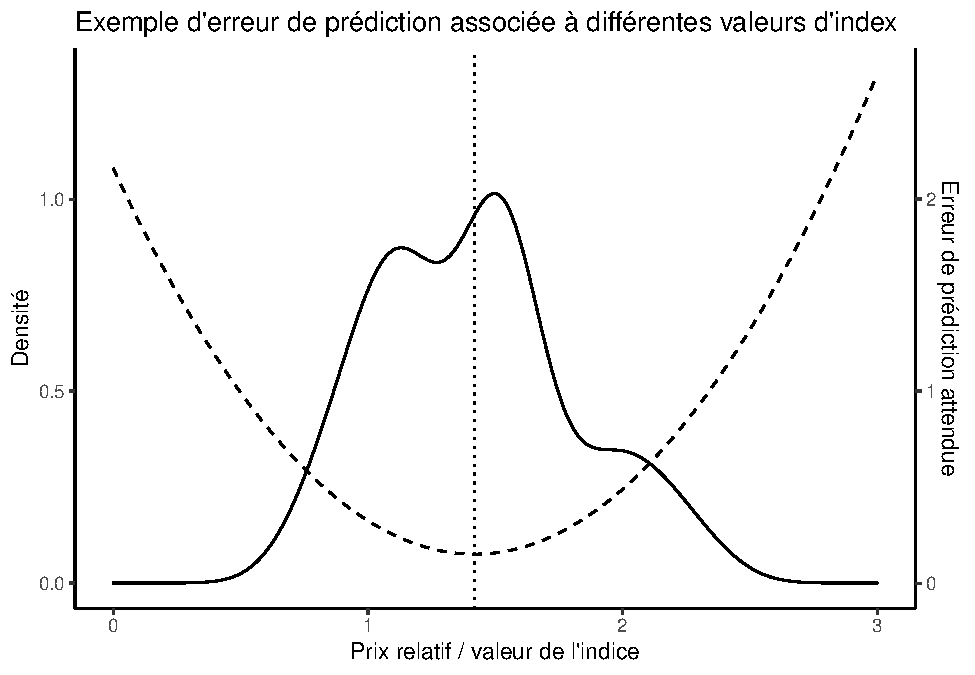
\includegraphics{cours-indices-des-prix_files/figure-latex/unnamed-chunk-10-1.pdf}

Comme la valeur attendue n'est qu'une moyenne pondérée, l'indice \(I^{A} = E(p_{t} / p_{0})\) est simplement un indice arithmétique qui fait la moyenne des prix relatifs. Ce qui est intéressant, c'est que les poids ont maintenant une nouvelle interprétation --- ils sont la probabilité d'observer un bien ou un service transigé dans la population. C'est,

\begin{align*}
I^{A} = \sum_{i = 1}^{n} \frac{p_{it}}{p_{i0}} P_{i}.
\end{align*}

Différentes formules arithmétiques d'indice de prix --- par exemple, Laspeyres, Paasche, Lowe --- correspondent donc à différentes déclarations sur ce qui détermine la probabilité d'observer une transaction. Par exemple, avec un indice de Laspeyres, les probabilités sont données par la part des dépenses ou des revenus de la période 0. Cela revient à dire que la probabilité d'observer une transaction pour un bien est la probabilité de dépenser ou de recevoir un dollar pour ce bien au cours de la période 0.

\hypertarget{indices-guxe9omuxe9triques-des-prix-1}{%
\subsection{Indices géométriques des prix}\label{indices-guxe9omuxe9triques-des-prix-1}}

Un indice géométrique peut être motivé de la même manière qu'un indice arithmétique. Formellement, un index géométrique est la valeur \(I^{G}\) qui résout

\begin{align*}
\min_{I} E\left[\left(\log\left(\frac{p_{t}} {p_{0}} \right) - \log(I) \right)^{2} \right] ,
\end{align*}

la solution à laquelle est \(I^{G} = \exp(E[\log (p_{t} / p_{0})])\). Mais ce n'est qu'un index géométrique, comme

\begin{align*}
\exp\left(E\left[\log \left(\frac{p_{t}} {p_{0}} \right) \right] \right) & = \exp \left(P_{i} \sum_{i = 1}^{n} \log \left(\frac{p_{it}} {p_{i0}} \right) \right) \\
&= \prod_{i = 1}^{n} \left(\frac{p_{it}}{p_{i0}} \right)^{P_{i}},
\end{align*}

avec des poids égaux à la probabilité d'observer un prix relatif. Il convient de noter qu'en raison des logarithmes du problème de prédiction, un indice géométrique peut également être motivé par la recherche d'une valeur \(I^{G}\) telle que \(I^{G} \times p_{i0}\) prédit le mieux \(p_{it}\) (ou \(p_{it} / I^{G}\) prédit le mieux \(p_{i0}\)). Il s'agit d'une propriété non partagée avec les indices arithmétiques. Alors qu'un indice arithmétique prédit les variations de prix au fil du temps, un indice géométrique prend le prix d'un bien pendant la période 0, le gonfle / le dégonfle avec l'indice des prix et utilise le résultat pour prédire le prix de ce bien pendant la période \(t\). Par conséquent, un indice géométrique s'intègre mieux dans l'approche stochastique car il correspond directement à la façon dont un indice des prix est utilisé pour gonfler et dégonfler les prix dans le temps dans la pratique.\footnote{Motiver un indice des prix pour résoudre le problème \(\min_{I} E[(p_{t} - p_{0} I)^{2}]\) donne \(I = E(p_{t} p_{0}) / E(p_{0}^{2})\), qui est un indice des prix assez inhabituel.}

L'indice de Törnqvist apparaît généralement comme le meilleur indice de l'approche stochastique car il sélectionne une valeur sensible pour représenter la probabilité d'observer un prix relatif. L'idée derrière les probabilités de Törnqvist est que la probabilité d'observer un prix particulier relatif à un bien dépend de la part des dépenses / revenus de ce bien sur les deux périodes. Ainsi, l'indice de Törnqvist définit les probabilités sous forme de parts de dépenses moyennes:

\begin{align*}
P_{i} = \frac{1}{2} \frac{p_{i0} q_{i0}}{\sum_{j = 1}^{n} p_{j0} q_{j0}} + \frac{1}{2} \frac{p_{it} q_{it}}{\sum_{j = 1}^{n} p_{jt} q_{jt}}.
\end{align*}

L'inconvénient de ces probabilités est qu'elles nécessitent des informations pour les parts des dépenses / recettes de la période 0 et de la période \(t\), ce qui peut ne pas être connu au moment du calcul de l'indice.

\hypertarget{des-indices-de-prix-plus-guxe9nuxe9raux}{%
\subsection{Des indices de prix plus généraux}\label{des-indices-de-prix-plus-guxe9nuxe9raux}}

Les indices arithmétiques et géométriques sont des cas particuliers d'une classe plus large d'indices de prix qui résolvent le problème de prédiction suivant:

\begin{align*}
\min_{I} E\left[\left(\left(\frac{p_{t}}{p_{0}} \right)^{r} - I^{r} \right)^{2} \right],
\end{align*}

pour certains \(r \neq 0\). La solution à ce problème est \(I = E((p_{t} / p_{0})^{r})^{1 / r}\). Fixer \(r = 1\) donne un indice arithmétique, alors que prendre \(r \rightarrow 0\) donne un indice géométrique (Bullen 2003, III 1 Theorem 2).

Ce qui est utile dans cette approche, c'est que de nombreux autres types d'indices de prix correspondent à différents choix de \(r\), et ceux-ci peuvent à leur tour être motivés pour résoudre un type de problème de prédiction. La définition de \(r = -1\), par exemple, produit un indice de prix harmonique

\begin{align*}
I^{H} = \left(\sum_{i = 1}^{n} \frac{P_{i}}{p_{it} / p_{i0}} \right)^{- 1}.
\end{align*}

Lorsque la probabilité d'observer un bien est donnée par sa part de dépenses période-\(t\), il s'agit de l'indice de Paasche. Fixer \(r = 1 - \sigma\), où \(\sigma\) est l'élasticité de substitution, donne l'indice de prix de Lloyd-Moulton

\begin{align*}
I^{LM} = \left(\sum_{i = 1}^{n} P_{i} \left(\frac{p_{it}}{p_{i0}} \right)^{1 - \sigma } \right)^{1 / (1 - \sigma)}
\end{align*}

lorsque les probabilités sont des dépenses / recettes pour la période 0.

Un point intéressant à propos de ces types d'indices de prix plus généraux est que, pour un ensemble de pondérations donné, la valeur de l'indice est plus grande lorsque le paramètre \(r\) augmente (Bullen 2003, III 3.1 Theorem 1). Cela donne le résultat familier qu'un indice arithmétique est plus grand qu'un indice géométrique, qui à son tour est plus grand qu'un indice harmonique, mais il peut également être utilisé pour classer des types d'indices plus exotiques comme l'indice Lloyd-Moulton.

\hypertarget{infuxe9rence-statistique}{%
\subsection{Inférence statistique}\label{infuxe9rence-statistique}}

Dans la pratique, la distribution complète des prix relatifs n'est généralement pas connue et un indice est calculé à partir d'un échantillon de prix collectés auprès des producteurs ou des détaillants. Cela signifie que les valeurs de l'indice sont calculées avec un estimateur pour \(I^{A}\) ou \(I^{G}\), selon qu'un indice arithmétique ou géométrique est l'indice cible. Bien que les sujets de l'échantillonnage et de l'inférence statistique se compliquent rapidement et dépassent le cadre de ce cours, il convient d'examiner comment les indices arithmétiques et géométriques se comportent lorsqu'ils sont calculés avec un échantillon aléatoire de données de prix.\footnote{Voir Balk (2008 Chapitre 5) pour une introduction à l'échantillonnage et à l'inférence statistique pour les indices de prix.} L'un des avantages de l'approche stochastique est qu'elle donne un aperçu du problème d'estimation d'un indice de prix avec un échantillon.

Avec l'échantillonnage aléatoire, une approche naturelle pour estimer l'indice arithmétique consiste à remplacer la valeur attendue --- une moyenne de population --- par la moyenne de l'échantillon. Cela donne un estimateur de la méthode des moments \(\hat {I}^A = 1 / n_{s} \sum_{i = 1}^{n_{s}} p_{it} / p_{i0}\), où \(n_{s}\) est la taille de l'échantillon, qui n'est qu'un index Carli. Si les parents de prix sont échantillonnés au hasard, alors il est facile de voir que \(E(\hat {I}^{A}) = I^{A}\), donc l'indice de Carli est un estimateur sans biais pour l'indice arithmétique.

Un estimateur naturel pour l'indice géométrique est \(\hat{I}^{G} = \prod_{i = 1}^{n_{s}} (p_{it} / p_{i0})^{1 / n_{s}}\), l'index Jevons. Contrairement à l'indice de Carli, cependant, l'indice de Jevons est un estimateur biaisé de l'indice géométrique. Il est à nouveau simple de montrer que \(E(\hat{I}^{G}) \geq I^{G}\), avec \(E(\hat{I}^{G}) = I^{G}\) ne tenant que dans des circonstances très particulières --- l'indice de Jevons surestime systématiquement l'indice géométrique (c'est-à-dire qu'il est biaisé à la hausse).\footnote{L'indice de Jevons n'est pas biaisé dans les cas où la distribution d'échantillonnage est dégénérée, ou la variance des prix relatifs est zéro. Voir Lehmann and Casella (1998 Chapitre 1 Théorème 7.5).} Bien que le biais soit un inconvénient de l'indice de Jevons, le biais n'est pas la seule propriété statistique importante d'un estimateur, et l'indice de Jevons a d'autres propriétés statistiques souhaitables (par exemple, c'est une constante estimateur de l'indice géométrique et, dans certaines circonstances, atteint le maximum d'efficacité de vraisemblance lié).\footnote{L'indice de Carli est également un estimateur cohérent de l'indice arithmétique sous échantillonnage aléatoire, mais il ne peut pas être un estimateur du maximum de vraisemblance car cela nécessiterait des prix apparentés d'avoir une distribution gaussienne, ce qui signifie que les prix relatifs peuvent être négatifs. En revanche, l'indice de Jevons est un estimateur du maximum de vraisemblance pour l'indice géométrique si les parents de prix ont une distribution log-normale, ce qui implique que les prix sont toujours positifs.} Il est possible d'ajuster le biais à la hausse des Jevons en divisant les Jevons index par \(1 + \sigma^{2} / (2n)\), où \(\sigma^{2}\) est la variance des logarithmes du prix (Kennedy 2003, 41), mais cela n'est généralement pas fait dans la pratique.

\hypertarget{affectation-1}{%
\section{Affectation}\label{affectation-1}}

Les réponses à ces questions proviennent à la fois du contenu du cours et des lectures. Chaque question vaut un point, pour un total de 20 points. La réussite de ce module nécessite au moins 65\% (13 sur 20 correct). Envoyez vos réponses par e-mail à l'instructeur du cours lorsque vous avez terminé.

\textbf{Question 1} Vrai ou faux: l'indice de Laspeyres est un indice du coût de la vie si les consommateurs ne se substituent pas à des produits plus chers lorsque les prix changent.

\textbf{Question 2} Vrai ou faux: le test d'inversion du temps indique qu'un indice des prix entre la période 0 et la période 1 est identique à l'inverse de l'indice des prix entre la période 1 et la période 0.

\textbf{Question 3} Quelle est la différence entre les approches économique et axiomatique des indices?

\begin{enumerate}
\def\labelenumi{\alph{enumi})}
\item
  Les prix et les quantités sont indépendants dans l'approche axiomatique et dépendants dans l'approche économique.
\item
  L'approche économique traite les prix comme fixes, tandis que l'approche axiomatique traite les prix comme aléatoires.
\item
  L'approche économique consiste en une série de tests basés sur la théorie économique pour évaluer la pertinence d'un numéro d'index, tandis que l'approche axiomatique utilise les axiomes fondamentaux de la théorie des ensembles pour évaluer dans quelle mesure un numéro d'index compare les listes de prix.
\item
  L'approche axiomatique et l'approche économique sont équivalentes.
\item
  Aucune de ces réponses.
\end{enumerate}

\textbf{Question 4} Quels poids l'indice Palgrave utilise-t-il pour agréger les prix relatifs entre la période 0 et la période 1?

\begin{enumerate}
\def\labelenumi{\alph{enumi})}
\item
  Part des dépenses / recettes de la période 0.
\item
  Part des dépenses / recettes de la période 1.
\item
  La moyenne géométrique des parts des dépenses / recettes de la période 0 et de la période 1.
\item
  La moyenne harmonique des parts des dépenses / recettes de la période 0 et de la période 1.
\item
  Aucune de ces réponses.
\end{enumerate}

\textbf{Question 5} Vrai ou faux: l'indice de Fisher est hautement considéré comme un numéro d'index car il satisfait aux axiomes les plus importants et correspond toujours à un indice du coût de la vie.

\textbf{Question 6} Vrai ou faux: le test d'inversion du temps indique qu'un indice de prix et un indice de quantité ont la même forme fonctionnelle.

\textbf{Question 7} Quel axiome l'indice Dutot ne satisfait-il pas?

\begin{enumerate}
\def\labelenumi{\alph{enumi})}
\item
  Monotonie.
\item
  Continuité.
\item
  Invariance dimensionnelle.
\item
  Circularité.
\item
  Aucune de ces réponses.
\end{enumerate}

\textbf{Question 8} Vrai ou faux: il est impossible qu'un indice géométrique de Laspeyres soit un indice du coût de la vie.

\textbf{Question 9} Quel type d'indice faut-il utiliser pour calculer un indice de quantité de Laspeyres en dégonflant la variation de la valeur globale entre deux périodes?

\begin{enumerate}
\def\labelenumi{\alph{enumi})}
\item
  Indice de Palgrave.
\item
  Indice de Laspeyres.
\item
  Indice de Paasche.
\item
  Indice de Fisher.
\item
  Indice géométrique de Laspeyres.
\end{enumerate}

\textbf{Question 10} Vrai ou faux: l'indice de Jevons est un estimateur biaisé de l'indice géométrique dans la population sous échantillonnage aléatoire.

Les 4 questions suivantes utilisent les données du tableau suivant qui contiennent une population de trois parents de prix, chacun avec une probabilité égale, et tous les échantillons possibles de cette population.

\begin{longtable}[]{@{}llll@{}}
\toprule
Population des parents de prix & Échantillon 1 & Échantillon 2 & Échantillon 3\tabularnewline
\midrule
\endhead
1.2 & 1.2 & 1.2 & 1.1\tabularnewline
1.1 & 1.1 & 1,35 & 1,35\tabularnewline
1,35 & \ldots{} & \ldots{} & \ldots{}\tabularnewline
\bottomrule
\end{longtable}

\textbf{Question 11} Quelle est la valeur de l'indice géométrique dans la population?

\begin{enumerate}
\def\labelenumi{\alph{enumi})}
\item
  121,2
\item
  100
\item
  120,5
\item
  129,8
\item
  98,7
\end{enumerate}

\textbf{Question 12} Quelle est la valeur moyenne (arithmétique) des indices de Jevons dans chaque échantillon?

\begin{enumerate}
\def\labelenumi{\alph{enumi})}
\item
  121,2
\item
  119,4
\item
  121,3
\item
  100
\item
  123,1
\end{enumerate}

\textbf{Question 13} Quelle est la valeur du biais dans l'indice de Jevons?

\begin{enumerate}
\def\labelenumi{\alph{enumi})}
\item
  0
\item
  -0,2
\item
  0,1
\item
  0,8
\item
  -1,3
\end{enumerate}

\textbf{Question 14} Quelle est la valeur du biais dans l'indice Carli?

\begin{enumerate}
\def\labelenumi{\alph{enumi})}
\item
  1,1
\item
  -0,4
\item
  -0,2
\item
  0,7
\item
  0
\end{enumerate}

\textbf{Question 15} Vrai ou faux: si un consommateur représentatif a une fonction d'utilité d'élasticité de substitution constante, l'ampleur du biais de substitution augmente à mesure que l'élasticité de substitution augmente.

Les quatre questions suivantes utilisent les données du tableau suivant qui contiennent des informations sur les prix et les quantités pour deux entrées sur deux périodes, ainsi qu'un véritable indice des prix des entrées.

\begin{longtable}[]{@{}llllll@{}}
\toprule
Période & Prix 1 & Prix 2 & Quantité 1 & Quantité 2 & Indice des prix des intrants\tabularnewline
\midrule
\endhead
0 & 100 & 60 & 141 & 391 & 100,0\tabularnewline
1 & 120 & 80 & 160 & 360 & 128,0\tabularnewline
\bottomrule
\end{longtable}

\textbf{Question 16} Quelle est la valeur de l'indice de Laspeyres?

\begin{enumerate}
\def\labelenumi{\alph{enumi})}
\item
  101,0
\item
  133,3
\item
  128,0
\item
  128,3
\item
  99,3
\end{enumerate}

\textbf{Question 17} Quelle est la valeur de l'indice de Paasche?

\begin{enumerate}
\def\labelenumi{\alph{enumi})}
\item
  127,7
\item
  131,2
\item
  101,0
\item
  99,1
\item
  130,0
\end{enumerate}

\textbf{Question 18} Quelle est la valeur de l'indice Jevons?

\begin{enumerate}
\def\labelenumi{\alph{enumi})}
\item
  120,1
\item
  128,2
\item
  99,0
\item
  126,5
\item
  98,4
\end{enumerate}

\textbf{Question 19} Vrai ou faux: l'indice Jevons calculé à la question 18 est plus proche de l'indice des prix des intrants que l'indice Fisher.

\textbf{Question 20} Vrai ou faux: il est possible de construire un indice des prix des intrants pour une entreprise qui détient un pouvoir de marché pour les produits qu'elle vend.

\hypertarget{part-construire-un-indice-des-prix-avec-r}{%
\part{Construire un indice des prix avec R}\label{part-construire-un-indice-des-prix-avec-r}}

\hypertarget{programme-2}{%
\section{Programme}\label{programme-2}}

La mise en pratique de la théorie de l'indice des prix nécessite des outils de calcul. Un outil particulièrement utile pour construire et analyser des indices de prix est le langage de programmation R.

L'objectif de ce module est de fournir une expérience pratique de la construction et de l'analyse d'un indice des prix avec R. À la fin de ce module, une personne devrait:

\begin{enumerate}
\def\labelenumi{\arabic{enumi}.}
\tightlist
\item
  Comprendre comment appliquer la théorie de l'indice des prix pour construire un indice des prix.
\item
  Savoir comparer les indices de prix de différentes sources.
\item
  Connaître la manière de construire et d'analyser un indice de prix avec R.
\end{enumerate}

Ce module est utile pour les compilateurs d'indices de prix ayant une compréhension de base de la théorie et de la construction d'un indice de prix, et qui souhaitent mettre la théorie en pratique et acquérir une compréhension plus approfondie de R.

Ce module consiste en une tâche de grande envergure qui permet aux apprenants de construire et d'analyser un indice de prix en R sur une semaine. Le rythme du module est autogéré, mais une semaine entière devrait être consacrée à ce travail. Toutes les données pour cette affectation ont été générées au hasard.

Prérequis: une introduction aux indices de prix et une compréhension de base de la théorie de l'indice des prix R. et des indices de prix de qualité constante, ainsi qu'une compréhension intermédiaire de R, sont utiles.

L'évaluation de ce module est basée sur une tâche unique qui s'appuie sur les connaissances antérieures des apprenants sur la théorie de l'indice des prix. Le devoir se compose de 4 questions (plus une question bonus). La collaboration sur la mission est encouragée, mais chaque personne doit soumettre son propre travail unique. Les réponses à la mission, ainsi que le code de travail pour chaque question (à l'exclusion de la question bonus) valent 15\%. L'instructeur doit être capable de comprendre et d'exécuter votre code; voir {[}example.R{]} (scripts / example.R) pour un exemple. Chaque question correctement répondue vaut 10\% supplémentaires. Répondre correctement à la question bonus vaut 20\%. La réussite de ce module nécessite une note de 60\% ou plus.

Veuillez envoyer un e-mail à l'instructeur du cours si vous avez des questions ou si vous avez besoin d'aide concernant le matériel ou le devoir du cours.

\hypertarget{affectation-2}{%
\section{Affectation}\label{affectation-2}}

Les widgets sont un produit fortement réglementé dans chacune des 10 provinces, et le gouvernement fédéral limite les mouvements de widgets entre les provinces. Récemment, en réponse au tollé général suscité par le caractère inaccessible des widgets, le groupe canadien d'analyse économique réglementaire a proposé que le gouvernement fédéral autorise le commerce interprovincial de widgets pour améliorer l'accès aux marchés et réduire les prix. Avant d'envisager de concevoir une nouvelle politique, le gouvernement fédéral aimerait toutefois évaluer comment les prix des widgets ont augmenté ces dernières années. Un indice des prix est nécessaire pour les marchés de widgets provinciaux et pour le pays dans son ensemble.

Le groupe Analyse réglementaire de la réglementation canadienne produit un indice mensuel des prix à l'échelle du Canada pour les widgets (c.-à-d.~Aucune ventilation provinciale), bien qu'il y ait peu d'information sur leurs sources de données ou leur méthodologie. La société privée Monsterweb, un courtier en widgets, établit également un indice des prix à l'échelle du Canada pour les widgets. Étant donné que les marchés provinciaux des widgets sont isolés les uns des autres, un indice des prix provincial est nécessaire pour évaluer comment les prix des widgets ont évolué au fil du temps et s'il est nécessaire que le gouvernement prenne des mesures politiques.

Les widgets sont de différents types, et une enquête a été utilisée pour collecter des devis mensuels pour une sélection de widgets représentatifs des types ``A'' à ``J'' de janvier 2018 à décembre 2019. Ces données sont stockées dans le système de prix globaux. Ces données d'enquête sont complétées par des données accessibles au public pour les transactions de widgets de type «K» qui n'ont pas pu être échantillonnées au cours de cette période, ainsi que la valeur des widgets traités dans chaque province en 2018 et 2019. Notez que les widgets de type «I» étaient un nouveau produit en 2019, et ces types de widgets ont remplacé les widgets de type ``J'' dans l'échantillon en 2019. En raison de la variation régionale des ventes de widgets, le même nombre de devis n'a pas pu être collecté pour tous les types de widgets dans toutes les provinces.

Toutes ces données sont résumées comme suit.

\begin{longtable}[]{@{}ll@{}}
\toprule
\begin{minipage}[b]{0.47\columnwidth}\raggedright
Nom de fichier\strut
\end{minipage} & \begin{minipage}[b]{0.47\columnwidth}\raggedright
Données\strut
\end{minipage}\tabularnewline
\midrule
\endhead
\begin{minipage}[t]{0.47\columnwidth}\raggedright
dat\_gps\strut
\end{minipage} & \begin{minipage}[t]{0.47\columnwidth}\raggedright
Offres de prix mensuelles pour les types de widget ``A'' à ``J'' de janvier 2018 à décembre 2019 à partir du système de prix globaux.\strut
\end{minipage}\tabularnewline
\begin{minipage}[t]{0.47\columnwidth}\raggedright
dat\_micro\strut
\end{minipage} & \begin{minipage}[t]{0.47\columnwidth}\raggedright
Microdonnées accessibles au public pour les transactions quotidiennes des widgets de type ``K'' de janvier 2018 à décembre 2019.\strut
\end{minipage}\tabularnewline
\begin{minipage}[t]{0.47\columnwidth}\raggedright
poids\strut
\end{minipage} & \begin{minipage}[t]{0.47\columnwidth}\raggedright
Valeur de la transaction de widget (en milliers de dollars) dans chaque province pour 2018 et 2019.\strut
\end{minipage}\tabularnewline
\begin{minipage}[t]{0.47\columnwidth}\raggedright
index\_crea\strut
\end{minipage} & \begin{minipage}[t]{0.47\columnwidth}\raggedright
L'indice des prix du groupe canadien d'analyse économique réglementaire.\strut
\end{minipage}\tabularnewline
\begin{minipage}[t]{0.47\columnwidth}\raggedright
index\_mw\strut
\end{minipage} & \begin{minipage}[t]{0.47\columnwidth}\raggedright
Indice des prix de Monsterweb.\strut
\end{minipage}\tabularnewline
\bottomrule
\end{longtable}

Votre objectif est de construire un indice mensuel des prix des widgets, de janvier 2018 à décembre 2019, pour chacune des 10 provinces et le pays dans son ensemble, et de valider cet indice avec ceux produits par le Groupe canadien d'analyse économique réglementaire et Monsterweb. Vous devrez utiliser cet index pour répondre aux questions suivantes.

\begin{enumerate}
\def\labelenumi{\arabic{enumi}.}
\item
  Quelle province a connu la plus forte augmentation des prix depuis le début de 2018? De combien les prix ont-ils changé?
\item
  Quelle province a connu la plus faible augmentation des prix depuis le début de 2018? De combien les prix ont-ils changé?
\item
  Quelle a été la plus importante variation des prix d'un mois à l'autre? Dans quelle province et quel mois cela s'est-il produit?
\item
  Tracez les trois indices au niveau du Canada sur un graphique. Quel indice montre la plus forte augmentation en pourcentage des prix des widgets nationaux depuis le premier trimestre 2019?
\item
  (Bonus) Calculez les coefficients de variation (CV) pour les indices provinciaux. En utilisant les règles de qualité habituelles pour la diffusion des données à Statistique Canada, quels indices provinciaux devraient être diffusés avec un avertissement (c.-à-d.~Un CV supérieur à 33,3)?
\end{enumerate}

\hypertarget{muxe9thodologie}{%
\subsection{Méthodologie}\label{muxe9thodologie}}

Les widgets vont être stratifiés par province et par type de widget pour produire des indices élémentaires au niveau de la province par type de widget. Ces indices élémentaires doivent être calculés avec un indice de Jevons. Les indices provinciaux et canadiens vont être des indices arithmétiques qui agrègent les indices élémentaires en utilisant des pondérations de part de valeur. Les pondérations des indices arithmétiques vont être mises à jour en 2019, avec janvier 2019 comme mois de liaison. La structure d'agrégation est résumée dans le graphique ci-dessous.

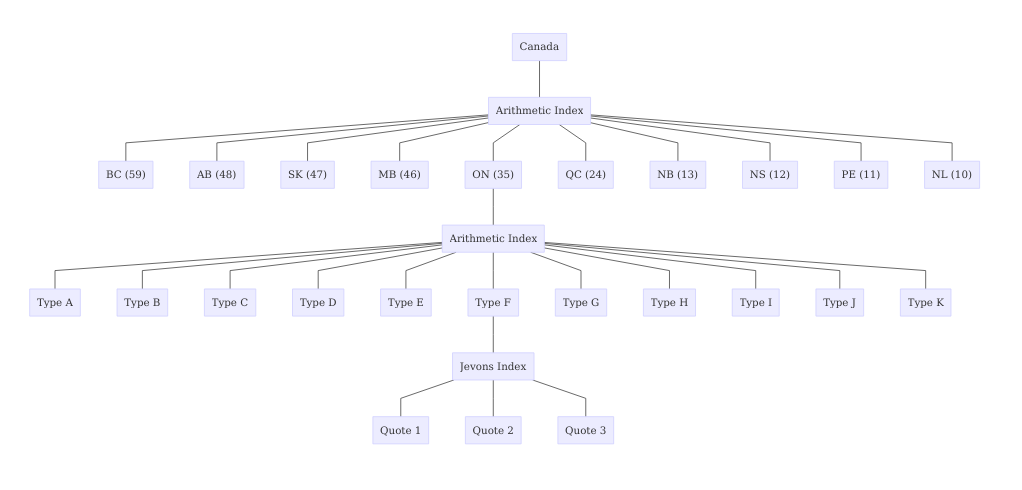
\includegraphics{img/structure.png}

\hypertarget{instructions}{%
\subsection{Instructions}\label{instructions}}

Ces instructions décrivent un moyen simple de construire l'indice des prix des widgets, mais n'hésitez pas à utiliser une approche différente si c'est plus facile. Le but est de comprendre le processus, plutôt que de concevoir le système le plus efficace en termes de calcul. (Astuce: consultez le package dplyr et le package \href{https://github.com/marberts/ppd}{ppd} pour quelques outils utiles.)

Exécutez le code suivant pour récupérer tous les fichiers de données et les placer dans votre environnement de travail.

\begin{Shaded}
\begin{Highlighting}[]
\KeywordTok{source}\NormalTok{ (}\StringTok{'https://raw.githubusercontent.com/ppd-dpp/price-index-course/master/scripts/get_data.R'}\NormalTok{)}
\end{Highlighting}
\end{Shaded}

\begin{enumerate}
\def\labelenumi{\arabic{enumi}.}
\item
  \textbf{Faites les poids}

  À l'aide du fichier «poids», créez un ensemble de poids qui donne la part de valeur de chaque produit vendu dans chaque province chaque année, et un autre qui donne la part de valeur de tous les produits vendus dans chaque province chaque année. Ce premier ensemble de poids sera utilisé pour agréger les indices élémentaires pour obtenir 10 indices au niveau de la province, et le deuxième ensemble de poids sera utilisé pour agréger les indices au niveau de la province en un indice national. Il devrait y avoir 200 poids dans le premier fichier et 20 poids dans le second fichier.
\item
  \textbf{Calculez la géomée du produit K}

  En utilisant les microdonnées pour le produit K dans le fichier \texttt{dat\_micro}, calculez la moyenne géométrique des prix dans chaque province pour chaque mois de chaque année de référence. Ce fichier devrait contenir 250 géomées.
\item
  \textbf{Calculez la géomée des produits A à J}

  En utilisant les données du système de prix globaux dans \texttt{dat\_gps}, calculez la moyenne géométrique des prix pour chaque produit dans chaque province dans chaque mois de chaque année de référence, pour les produits A à J. Combinez ces données avec les données préparées à l'étape 2. Le fichier résultant devrait avoir 2 500 géomées.
\item
  \textbf{Calculer les indices élémentaires période sur période}

  Pour chaque produit dans chaque province dans chaque année de référence, calculez le rapport des moyennes géométriques calculées à l'étape 3, en vous assurant d'avoir un prix relatif de 1 en janvier 2018 et janvier 2019 (janvier 2019 sera le mois de liaison lorsqu'il est le temps de chaîner l'index.)
\item
  \textbf{Prix mettre à jour les poids des produits}

  Fusionnez les pondérations au niveau du produit par province de l'étape 1 dans l'ensemble de données créé à l'étape 4 et utilisez les indices élémentaires période sur période pour mettre à jour les pondérations.
\item
  \textbf{Calculez l'indice provincial}

  Calculez un indice arithmétique pour chaque province au cours de chaque année de référence, à l'aide des indices élémentaires d'une période à l'autre et des pondérations mises à jour des prix des étapes 4 et 5.
\item
  \textbf{Calculez l'indice au niveau du Canada}

  Fusionnez les pondérations provinciales à l'étape 1 avec les indices provinciaux de l'étape 6 pour calculer un indice canadien pour chaque année de référence.
\item
  \textbf{Chaîne des indices 2018 et 2019}

  Enchaînez les indices au niveau de la province de 2018 et 2019 et du niveau du Canada ensemble, en utilisant janvier 2019 comme mois de liaison, pour obtenir un indice de janvier 2018 à décembre 2019 avec janvier 2018 comme période de base (généralement, la période de base serait une année civile , mais il n'y a que 24 mois de données).
\end{enumerate}

Le résultat final devrait être un fichier avec 11 indices de prix, un pour chaque province et un indice national, de janvier 2018 à décembre 2019, avec janvier 2018 comme période de base (= 100).

La validation de l'indice au niveau du Canada nécessite de mettre l'indice du groupe canadien d'analyse économique réglementaire et l'indice Monsterweb sous une forme commune.

\begin{enumerate}
\def\labelenumi{\arabic{enumi}.}
\setcounter{enumi}{8}
\item
  \textbf{Trimestre par rapport aux indices mensuels}

  Transformez l'indice que vous venez de créer et l'indice du groupe Analyse réglementaire de la réglementation canadienne dans \texttt{index\_crea} en un indice trimestriel, avec le 1er trimestre 2019 comme période de base, en prenant la moyenne des trois valeurs d'indice de chaque trimestre.
\item
  \textbf{Ajoutez les trois indices ensemble}

  Rassemblez les indices de l'étape 9 dans un ensemble de données avec l'index de Monsterweb dans \texttt{index\_mw}. Ils devraient tous être trimestriels avec le premier trimestre 2019 comme période de base (= 100).
\end{enumerate}

\hypertarget{ruxe9fuxe9rences}{%
\section*{Références}\label{ruxe9fuxe9rences}}
\addcontentsline{toc}{section}{Références}

\hypertarget{refs}{}
\leavevmode\hypertarget{ref-balk1995}{}%
Balk, B. M. 1995. ``Axiomatic Price Index Theory: A Survey.'' \emph{International Statistical Review/Revue Internationale de Statistique} 63 (1): 69--93.

\leavevmode\hypertarget{ref-balk2008}{}%
---------. 2008. \emph{Price and Quantity Index Numbers}. Cambridge University Press.

\leavevmode\hypertarget{ref-balk2001}{}%
Balk, B. M., and W. E. Diewert. 2001. ``A Characterization of the Törnqvist Price Index.'' \emph{Economics Letters} 72 (3): 279--81.

\leavevmode\hypertarget{ref-bullen2003}{}%
Bullen, P. S. 2003. \emph{Handbook of Means and Their Inequalities}. Springer.

\leavevmode\hypertarget{ref-cpimanual}{}%
ILO, IMF, OECD, Eurostat, UN, and World Bank. 2004a. \emph{Consumer Price Index Manual: Theory and Practice}. International Monetary Fund.

\leavevmode\hypertarget{ref-ppimanual}{}%
---------. 2004b. \emph{Producer Price Index Manual: Theory and Practice}. International Monetary Fund.

\leavevmode\hypertarget{ref-kennedy2003}{}%
Kennedy, P. 2003. \emph{A Guide to Econometrics}. 5th ed. MIT University Press.

\leavevmode\hypertarget{ref-kirman1992}{}%
Kirman, A. P. 1992. ``Whom or What Does the Representative Individual Represent?'' \emph{Journal of Economic Perspectives} 6 (2): 117--36.

\leavevmode\hypertarget{ref-lehmann1998}{}%
Lehmann, E. L., and G. Casella. 1998. \emph{Theory of Point Estimation}. 2nd ed. Springer.

\leavevmode\hypertarget{ref-lord2002}{}%
Lord, N. 2002. ``Does Smaller Spread Always Mean Larger Product?'' \emph{The Mathematical Gazette} 86 (506): 273--74.

\leavevmode\hypertarget{ref-martin2019}{}%
Martin, S. 2019. ``Moral Management in Competitive Markets.'' \emph{Journal of Economics \& Management Strategy} 28 (3): 541--60.

\leavevmode\hypertarget{ref-mcfadden1978}{}%
McFadden, D. 1978. ``Cost, Revenue, and Profit Functions.'' In \emph{Production Economics: A Dual Approach to Theory and Applications}, edited by M. Fuss and D. McFadden. North-Holland.

\leavevmode\hypertarget{ref-pollak1980}{}%
Pollak, R. A. 1980. ``Group Cost-of-Living Indexes.'' \emph{The American Economic Review} 70 (2): 273--78.

\end{document}
